\subsection{Berechnung: Analytischen Lösung der Modellierung}\label{Lösung}
In diesem Abschnitt werden die Gleichungen \ref{eq:34}, \ref{eq:35} und \ref{eq:36} herlgeleitet:
\begin{itemize}
	\item Aus Gleichung \ref{eq:11} und \ref{eq:22} ergibt sich:
	\begin{equation}\label{eq:164}
		R_{4}=0
	\end{equation}
	\item Aus Gleichung \ref{eq:9} und \ref{eq:23} ergibt sich:
	\begin{equation}\label{eq:165}
		R_{2}=0
	\end{equation}
	\item Aus Gleichung \ref{eq:18} und \ref{eq:33} ergibt sich:
	\begin{equation}\label{eq:166}
		R_{9}=-F
	\end{equation}
	\item Aus Gleichung \ref{eq:13}, \ref{eq:18}, \ref{eq:33} und \ref{eq:166} ergibt sich:
	\begin{equation}\label{eq:167}
		R_{5}=-F_{pruef}-F_{Q}
	\end{equation}
	\item Aus Gleichung \ref{eq:19} , \ref{eq:32} und \ref{eq:166} ergibt sich:
	\begin{equation}\label{eq:168}
		R_{10}=F_{pruef}\cdot (l_{1}+l_{2}+l_{3})
	\end{equation}
	\item Aus Gleichung \ref{eq:14}, \ref{eq:19}, \ref{eq:30}, \ref{eq:166}, \ref{eq:167} und \ref{eq:168} ergibt sich:
	\begin{equation}\label{eq:169}
		R_{6}=F_{pruef}\cdot (l_{1}+l_{2}+l_{3}) + F_{Q}\cdot (l_{1}+l_{2})
	\end{equation}
	\item Aus Gleichung \ref{eq:9}, \ref{eq:14}, \ref{eq:27}, \ref{eq:167} und \ref{eq:169} ergibt sich:
	\begin{equation}\label{eq:170}
		R_{1}=F_{pruef}\cdot\frac{l_{2}+l_{3}}{l_{1}} + F_{Q}\cdot\frac{l_{2}}{l_{1}}
	\end{equation}
	\item Aus Gleichung \ref{eq:11}, \ref{eq:24} und \ref{eq:170} ergibt sich:
	\begin{equation}\label{eq:171}
		R_{3}=-\frac{1}{6}\cdot F_{pruef}\cdot (l_{2}+l_{3})\cdot l_{1} - \frac{1}{6}\cdot F_{Q}\cdot l_{2}\cdot l_{1}
	\end{equation}
	\item Aus Gleichung \ref{eq:10}, \ref{eq:15}, \ref{eq:26}, \ref{eq:167}, \ref{eq:169}, \ref{eq:170} und \ref{eq:171} ergibt sich:
	\begin{equation}\label{eq:172}
		R_{7}=F_{pruef}\cdot \Bigl(-\frac{1}{2} l_{1}^{2}-\frac{2}{3} l_{1}l{2}-\frac{2}{3} l_{1}l{3}\Bigr) + F_{Q}\cdot \Bigl(-\frac{1}{2} l_{1}^{2}-\frac{2}{3} l_{1}l{2}\Bigr)
	\end{equation}
	\item Aus Gleichung \ref{eq:16}, \ref{eq:25}, \ref{eq:167}, \ref{eq:169} und \ref{eq:172} ergibt sich:
	\begin{equation}\label{eq:173}
		R_{8}=F_{pruef}\cdot \Bigl(\frac{1}{6} l_{1}^{3}+\frac{1}{6} l_{1}^{2}l{2}+\frac{1}{6} l_{1}^{2}l{3}\Bigr) + F_{Q}\cdot \Bigl(\frac{1}{6} l_{1}^{3}+\frac{1}{6} l_{1}^{2}l{2}\Bigr)
	\end{equation}
	\item Aus Gleichung \ref{eq:15}, \ref{eq:20}, \ref{eq:29}, \ref{eq:166}, \ref{eq:167}, \ref{eq:168}, \ref{eq:169} und \ref{eq:172} ergibt sich:
	\begin{equation}\label{eq:174}
		R_{11}=F_{pruef}\cdot \Bigl(-\frac{1}{2} l_{1}^{2}-\frac{2}{3} l_{1}l{2}-\frac{2}{3} l_{1}l{3}\Bigr) + F_{Q}\cdot \Bigl(\frac{1}{2} l_{1}^{2}+\frac{1}{3} l_{1}l{2}\Bigr)
	\end{equation}
	\item Aus Gleichung \ref{eq:16}, \ref{eq:21}, \ref{eq:28}, \ref{eq:166}, \ref{eq:167}, \ref{eq:168}, \ref{eq:169}, \ref{eq:172}, \ref{eq:173} und \ref{eq:174} ergibt sich:
	\begin{equation}\label{eq:175}
		R_{12}=F_{pruef}\cdot \Bigl(\frac{1}{6} l_{1}^{3}+\frac{1}{6} l_{1}^{2}l{2}+\frac{1}{6} l_{1}^{2}l{3}\Bigr) + F_{Q}\cdot \Bigl(\frac{1}{6} l_{2}^{3}-\frac{1}{3} l_{1}^{2}l{2}-\frac{1}{2} l_{2}^{2}l{1}\Bigr)
	\end{equation}
	\item Nun können die Gleichungen \ref{eq:166}, \ref{eq:167}, und \ref{eq:170} in folgende Gleichung eingesetzt werden, sodass sich Gleichung \ref{eq:34} ergibt:
	\begin{equation}
		Q(y,F_{pruef},F_{Q},EI_{x})=\left\{\begin{array}{ll}
			-R_{1}&,y\epsilon (0,l_{1})\\
			-R_{5}&,y\epsilon (l_{1}, l_{1}+l_{2})\\
			-R_{9}&,y\epsilon (l_{1}+l_{2}, l_{1}+l_{2}+l_{3})
		\end{array}\right.
	\end{equation}
	\item Nun können die Gleichungen \ref{eq:165}, \ref{eq:166}, \ref{eq:167}, \ref{eq:168}, \ref{eq:169} und \ref{eq:170} in folgende Gleichung eingesetzt werden, sodass sich Gleichung \ref{eq:35} ergibt:
	\begin{equation}
		M(y,F_{pruef},F_{Q},EI_{x})=\left\{\begin{array}{ll}
			-R_{1}\cdot y - R_{2}&,y\epsilon (0,l_{1})\\
			-R_{5}\cdot y - R_{6}&,y\epsilon (l_{1}, l_{1}+l_{2})\\
			-R_{9}\cdot y - R_{10}&,y\epsilon (l_{1}+l_{2}, l_{1}+l_{2}+l_{3})
		\end{array}\right.
	\end{equation}
	\item Nun können die Gleichungen  \ref{eq:164}, \ref{eq:165}, \ref{eq:166}, \ref{eq:167}, \ref{eq:168}, \ref{eq:169}, \ref{eq:170},  \ref{eq:171},  \ref{eq:172},  \ref{eq:172},  \ref{eq:174} und  \ref{eq:175} in folgende Gleichung eingesetzt werden, sodass sich Gleichung \ref{eq:36} ergibt:
	\begin{equation}
		w(y,F_{pruef},F_{Q},EI_{x})=\left\{\begin{array}{ll}
			\frac{1}{EI}\cdot\Bigl(\frac{R_{1}\cdot y^{3}}{6}+\frac{R_{2}\cdot y^{2}}{2}+R_{3}\cdot y +R_{4}\Bigr)&,y\epsilon (0,l_{1})\\
			\frac{1}{EI}\cdot\Bigl(\frac{R_{5}\cdot y^{3}}{6}+\frac{R_{6}\cdot y^{2}}{2}+R_{7}\cdot y +R_{8}\Bigr)&,y\epsilon (l_{1}, l_{1}+l_{2})\\
			\frac{1}{EI}\cdot\Bigl(\frac{R_{9}\cdot y^{3}}{6}+\frac{R_{10}\cdot y^{2}}{2}+R_{11}\cdot y +R_{12}\Bigr)&,y\epsilon (l_{1}+l_{2}, l_{1}+l_{2}+l_{3})
		\end{array}\right.
	\end{equation}
\end{itemize}
\newpage
\subsection{Berechung: Schubfluss und Schubmittelpunkt}
\begin{itemize}
	\item Wertebereich der Laufvariable
	\begin{center}
		\begin{tabular}[h]{l|c|c}
			$i$&$s_i\in(0,...)$\\
			\hline
			1&58,90\\
			2&14,00\\
			3&37,50\\
			4&14,00\\
			5&107,72\\
			6&30,07\\
			7&83,46\\
			8&14\\
			9&14\\
			10&37,5\\
		\end{tabular}
	\end{center}
	\item Statische Momente im allgemeinen Koordinatensystem mit $s_0$: (Werte sind aus Abb. \ref{Fluegel1} zu entnehmen)
	%1
	\begin{equation}
		S_{z,1}(s_1) = t\int_{0}^{s_1} R\bigg(1-cos\bigg(\frac{s}{R}\bigg)\bigg)ds = tR^2\bigg[\frac{s}{R} - sin\bigg(\frac{s}{R}\bigg)\bigg]_{s=0}^{s_1} = tR^2\cdot\bigg(\frac{s_1}{R}-sin\bigg(\frac{s_1}{R}\bigg)\bigg)
	\end{equation}
	\begin{equation}
		S_{y,1}(s_1) = t\int_{0}^{s_1} -Rsin\bigg(\frac{s}{R}\bigg)ds_1 = t\biggl[ R^2 cos\bigg(\frac{s}{R}\bigg)\biggr]^{s_1}_{s=0} = tR^2 \cdot\bigg(cos\bigg(\frac{s_1}{R}\bigg)-1\bigg)
	\end{equation}
%2
\begin{equation}
	\begin{split}
		S_{z,2}(s_2) &= t\int_{0}^{s_2}\bigg(37,5\mathrm{mm}+cos(\alpha)\cdot s\bigg)ds + S_{z,1}(s_{1,\mathrm{ende}}) \\\
		&= t\bigg[37,5\mathrm{mm}\cdot s +\frac{cos(\alpha)}{2}\cdot s^2_2\bigg]_{s=0}^{s_2} + S_{z,1}(s_{1,\mathrm{ende}}) \\\ 
		&= t\cdot\bigg(37,5\mathrm{mm}\cdot s_2 +\frac{cos(\alpha)}{2}\cdot s^2_2\bigg) + S_{z,1}(s_{1,\mathrm{ende}})
	\end{split}
\end{equation}
\begin{equation}
	\begin{split}
		S_{y,2}(s_2) &= t\int_{0}^{s_2}\bigg(-37,5\mathrm{mm}+sin(\alpha)\cdot s\bigg)ds + S_{y,1}(s_{1,\mathrm{ende}}) \\\
		&= t\bigg[-37,5\mathrm{mm}\cdot s +\frac{sin(\alpha)}{2}\cdot s^2\bigg]_{s=0}^{s_2} + S_{y,1}(s_{1,\mathrm{ende}})\\\
		&= t\cdot\bigg(-37,5\mathrm{mm}\cdot s_2 +\frac{sin(\alpha)}{2}\cdot s^2_2\bigg) + S_{y,1}(s_{1,\mathrm{ende}})
	\end{split}
\end{equation}
%3
\begin{equation}
	S_{z,3}(s_3) = t_1\int_{0}^{s_3}\bigg(37,5\mathrm{mm}+14\mathrm{mm}\bigg)ds = t_1\bigg[51,5\mathrm{mm}\cdot s\bigg]_{s=0}^{s_3} = t_1\cdot\bigg(51,5\mathrm{mm}\cdot s_3\bigg)
\end{equation}
\begin{equation}
	S_{y,3}(s_3) = t_1\int_{0}^{s_3}-s\ ds= t_1\bigg[-\frac{1}{2}s^2\bigg]_{s=0}^{s_3} = t_1\cdot\bigg(-\frac{1}{2}s^2_3\bigg)
\end{equation}
%4
\begin{equation}
\begin{split}
	S_{z,4} &= t\int_{0}^{s_4}\bigg(37,5\mathrm{mm}+cos(\alpha)(s_{2,\mathrm{ende}}+s)\bigg)ds + S_{z,2}(s_{2,\mathrm{ende}})  + S_{z,3}(s_{3,\mathrm{ende}})\\\
	&= t\bigg[51,37\mathrm{mm}\cdot s + \frac{1}{2}s^2\bigg]_{s=0}^{s_4} + S_{z,2}(s_{2,\mathrm{ende}})  + S_{z,3}(s_{3,\mathrm{ende}})\\\
	&= t\cdot\bigg(51,37\mathrm{mm}\cdot s_4 + \frac{1}{2}s^2_4\bigg) + S_{z,2}(s_{2,\mathrm{ende}})  + S_{z,3}(s_{3,\mathrm{ende}})
\end{split}
\end{equation}
\begin{equation}
\begin{split}
	S_{y,4} &= t\int_{0}^{s_4}\bigg(-37,5\mathrm{mm}+sin(\alpha)(s_{2,\mathrm{ende}}+s)\bigg)ds + S_{y,2}(s_{2,\mathrm{ende}})  + S_{y,3}(s_{3,\mathrm{ende}})\\\
	&= t\bigg[-35,63\mathrm{mm}\cdot s + \frac{1}{2}s^2\bigg]_{s=0}^{s_4} + S_{y,2}(s_{2,\mathrm{ende}})  + S_{y,3}(s_{3,\mathrm{ende}})\\\
	&= t\cdot\bigg(-35,62\mathrm{mm}\cdot s_4 + \frac{1}{2}s^2_4\bigg) + S_{y,2}(s_{2,\mathrm{ende}})  + S_{y,3}(s_{3,\mathrm{ende}})
\end{split}
\end{equation}
%5
\begin{equation}
	\begin{split}
		S_{z,5} &= t\int_{0}^{s_5}\bigg(37,5\mathrm{mm}+cos(\alpha)(s_{2,\mathrm{ende}}+s_{4,\mathrm{ende}}+s)\bigg)ds + S_{z,4}(s_{4,\mathrm{ende}})\\\
		&= t\bigg[65,25\mathrm{mm}\cdot s +\frac{1}{2}s^2\bigg]_{s=0}^{s_5} + S_{z,4}(s_{4,\mathrm{ende}})\\\
		&= t\cdot\bigg(65,25\mathrm{mm}\cdot s_5 +\frac{1}{2}s^2_5\bigg) + S_{z,4}(s_{4,\mathrm{ende}})
	\end{split}
\end{equation}
\begin{equation}
	\begin{split}
		S_{y,5} &= t\int_{0}^{s_5}\bigg(-37,5\mathrm{mm}+sin(\alpha)(s_{2,\mathrm{ende}}+s_{4,\mathrm{ende}}+s)\bigg)ds + S_{y,4}(s_{4,\mathrm{ende}})\\\
		&= t\bigg[-33,75\mathrm{mm}\cdot s +\frac{1}{2}s^2\bigg]_{s=0}^{s_5} + S_{y,4}(s_{4,\mathrm{ende}})\\\
		&= t\cdot\bigg(-33,75\mathrm{mm}\cdot s_5 +\frac{1}{2}s^2_5\bigg) + S_{y,4}(s_{4,\mathrm{ende}})
	\end{split}
\end{equation}
%6
\begin{equation}
	\begin{split}
		S_{z,6} &= t\int_{0}^{s_6}\bigg(172\mathrm{mm}-cos(\beta)\cdot s\bigg)ds + S_{z,5}(s_{5,\mathrm{ende}})\\\
		&= t\bigg[172\mathrm{mm}\cdot s-\frac{cos(\beta)}{2}\cdot s^2\bigg]_{s=0}^{s_6} + S_{z,5}(s_{5,\mathrm{ende}})\\\
		&= t\cdot\bigg(172\mathrm{mm}\cdot s_6-\frac{cos(\beta)}{2}\cdot s^2_6\bigg) + S_{z,5}(s_{5,\mathrm{ende}})
	\end{split}
\end{equation}
\begin{equation}
	\begin{split}
	S_{y,6} &= t\int_{0}^{s_6}\bigg(sin(\beta)\cdot(s-s_{6,\mathrm{ende}})\bigg)ds + S_{y,5}(s_{5,\mathrm{ende}})\\\
	&= t\bigg[-19,33\mathrm{mm}\cdot s + \frac{sin(\beta)}{2}\cdot s^2\bigg]_{s=0}^{s_6} + S_{y,5}(s_{5,\mathrm{ende}})\\\
	&= t\cdot\bigg(-19,33\mathrm{mm}\cdot s_6 + \frac{sin(\beta)}{2}\cdot s^2_6\bigg) + S_{y,5}(s_{5,\mathrm{ende}})
	\end{split})
\end{equation}
%7
\begin{equation}
	\begin{split}
		S_{z,7} &= t\int_{0}^{s_7}\bigg(172\mathrm{mm}-cos(\beta)s_{6,\mathrm{ende}}-s\bigg)ds + S_{z,6}(s_{6,\mathrm{ende}})\\\
		&= t\bigg[148,96\mathrm{mm}\cdot s-\frac{1}{2}s^2\bigg]_{s=0}^{s_7} + S_{z,6}(s_{6,\mathrm{ende}})\\\
		&= t\cdot\bigg(148,96\mathrm{mm}\cdot s_7-\frac{1}{2}s^2_7\bigg) + S_{z,6}(s_{6,\mathrm{ende}})
	\end{split}
\end{equation}
\begin{equation}
	S_{y,7} = t\int_{0}^{s_7}0\ ds + S_{y,6}(s_{6,\mathrm{ende}}) = S_{y,6}(s_{6,\mathrm{ende}})
\end{equation}
%8
\begin{equation}
\begin{split}
	S_{z,8} &= t\int_{0}^{s_8}\bigg(172\mathrm{mm}-cos(\beta)s_{6,\mathrm{ende}}-s_{7,\mathrm{ende}}-s\bigg)ds + S_{z,7}(s_{7,\mathrm{ende}})\\\
	&= t\bigg[65,5\mathrm{mm}\cdot s-\frac{1}{2}s^2\bigg]_{s=0}^{s_8} + S_{z,7}(s_{7,\mathrm{ende}})\\\
	&= t\cdot\bigg(65,5\mathrm{mm}\cdot s_8-\frac{1}{2}s^2_8\bigg) + S_{z,7}(s_{7,\mathrm{ende}})
\end{split}
\end{equation}
\begin{equation}
	S_{y,8} = t\int_{0}^{s_8}0\ ds + S_{y,7}(s_{7,\mathrm{ende}}) =S_{y,7}(s_{7,\mathrm{ende}})
\end{equation}
%9
\begin{equation}
		\begin{split}
		S_{z,9} &= t\int_{0}^{s_9}\bigg(172\mathrm{mm}-cos(\beta)s_{6,\mathrm{ende}}-s_{7,\mathrm{ende}}-s_{8,\mathrm{ende}}-s\bigg)ds + S_{z,8}(s_{8,\mathrm{ende}})\\\
		&= t\bigg[51,5\mathrm{mm}\cdot s-\frac{1}{2}s^2\bigg]_{s=0}^{s_9} + S_{z,8}(s_{8,\mathrm{ende}})\\\
		&= t\cdot\bigg(51,5\mathrm{mm}\cdot s_9-\frac{1}{2}s^2_9\bigg) + S_{z,8}(s_{8,\mathrm{ende}})
	\end{split}
\end{equation}
\begin{equation}
	S_{y,9} = t\int_{0}^{s_9}0\ ds + S_{y,8}(s_{8,\mathrm{ende}}) = S_{y,8}(s_{8,\mathrm{ende}})
\end{equation}
%10
\begin{equation}
	\begin{split}
		S_{z,10} &= t\int_{0}^{s_{10}}\bigg(172\mathrm{mm}-cos(\beta)s_{6,\mathrm{ende}}-s_{7,\mathrm{ende}}-s_{8,\mathrm{ende}}-s_{9,\mathrm{ende}}-s\bigg)ds + S_{z,9}(s_{9,\mathrm{ende}})\\\
		&= t\bigg[37,5\mathrm{mm}\cdot s - \frac{1}{2}s^2\bigg]_{s=0}^{s_10} + S_{z,9}(s_{9,\mathrm{ende}})\\\
		&= t\cdot\bigg(37,5\mathrm{mm}\cdot s_10 - \frac{1}{2}s^2\bigg) + S_{z,9}(s_{9_10,\mathrm{ende}})
	\end{split}
\end{equation}
\begin{equation}
	S_{y,10} = t\int_{0}^{s_{10}}0\ ds + S_{z,9}(s_{9,\mathrm{ende}}) = S_{z,9}(s_{9,\mathrm{ende}})
\end{equation}
	\item Hebelarme um den Pol unter Berücksichtigung des positiven Drehsinnes
		\begin{center}
		\begin{tabular}[h]{l|c|c}
			$i$&$r_i\mathrm{/mm}$\\
			\hline
			1&37,5\\
			2&37,16\\
			3&-14\\
			4&37,16\\
			5&37,16\\
			6&81,97\\
			7&0\\
			8&0\\
			9&0\\
			10&0\\
		\end{tabular}
	\end{center}
	\item Integrale über Statische Momente mit $t=0,2$mm
	\begin{equation}
		S_{\bar z}(s) = S_z(s) - y_0ts
	\end{equation}
	\begin{equation}
		S_{\bar y}(s) = S_y(s) - z_0ts
	\end{equation}
~\\%1
	\begin{equation}
		\begin{split}
			\int S_{\bar z,1}\ ds_1 &= \int  tR^2\cdot\bigg(\frac{s_1}{R}-sin\bigg(\frac{s_1}{R}\bigg)-\frac{y_0s_1}{R^2}\bigg)\ ds_1\\\
			&=tR^3\bigg[\frac{s_1^2}{2R^2}\bigg(1-\frac{y_0}{R}\bigg)+cos\bigg(\frac{s_1}{R}\bigg)\bigg]_{s_1=0}^{s_{1,\mathrm{ende}}} = -24781,04\mathrm{mm}^4
		\end{split}
	\end{equation}
	\begin{equation}
		\begin{split}
			\int S_{\bar y,1}\ ds_1 &= \int tR^2 \cdot\bigg(cos\bigg(\frac{s_1}{R}\bigg)-1 - \frac{z_0s_1}{R^2}\bigg)\ ds_1\\\
			&=tR^3\bigg[sin\bigg(\frac{s_1}{R}\bigg) -\frac{s_1}{R} - \frac{z_0s_1^2}{2R^3}\bigg]_{s_1=0}^{s_{1,\mathrm{ende}}} = -679,64\mathrm{mm}^4
		\end{split}
	\end{equation}
%2
	\begin{equation}
		\begin{split}
			\int S_{\bar z,2}\ ds_2 &= \int  \bigg(t\cdot\bigg(37,5\mathrm{mm}\cdot s_2 +\frac{cos(\alpha)}{2}\cdot s^2_2\bigg) + S_{z,1}(s_{1,\mathrm{ende}})-y_0ts_2\bigg)\ ds_2\\\
			&=\bigg[t\bigg(s_2^2\frac{37,5\mathrm{mm}-y_0}{2}+\frac{cos(\alpha)}{6}\cdot s^3_2\bigg)+S_{z,1}(s_{1,\mathrm{ende}})s_2\bigg]_{s_2=0}^{s_{2,\mathrm{ende}}}\\\
			&= -11417,94\mathrm{mm}^4
		\end{split}
	\end{equation}
	\begin{equation}
		\begin{split}
			\int S_{\bar y,2}\ ds_2 &= \int\bigg( t\cdot\bigg(-37,5\mathrm{mm}\cdot s_2 +\frac{sin(\alpha)}{2}\cdot s^2_2\bigg) + S_{y,1}(s_{1,\mathrm{ende}}) - z_0ts_2\bigg)\ ds_2\\\
			&= \bigg[t\bigg(-s_2^2\frac{37,5\mathrm{mm}+z_0}{2}+\frac{sin(\alpha)}{6}s_2^3\bigg)+S_{y,1}(s_{1,\mathrm{ende}})s_2\bigg]_{s_2=0}^{s_{2,\mathrm{ende}}}\\\
			&=-1819,86\mathrm{mm}^4
		\end{split}
	\end{equation}
%3
	\begin{equation}
		\begin{split}
			\int S_{\bar z,3}\ ds_3 &= \int \bigg(t_1\cdot\bigg(51,5\mathrm{mm}\cdot s_3\bigg) -y_0t_1s_3\bigg)\ ds_3\\\
			&=t_1\bigg[\frac{51,5\mathrm{mm}-y_0}{2}s_3^2\bigg]_{s_3=0}^{s_{3,\mathrm{ende}}}\\\
			&=-5967,72\mathrm{mm}^4
		\end{split}
	\end{equation}
	\begin{equation}
		\begin{split}
			\int S_{\bar y,3}\ ds_3 &= \int t_1\cdot\bigg(-\frac{1}{2}s^2_3-z_0s_3\bigg)\ ds_3\\\
			&=t_1\bigg[-\frac{s_3^3}{6}-\frac{z_0}{2}s_3^2\bigg]\\\
			&=638,06\mathrm{mm}^4
		\end{split}
	\end{equation}
%4
	\begin{equation}
		\begin{split}
			\int S_{\bar z,4}\ ds_4 &= \int \bigg(t\cdot\bigg(-35,62\mathrm{mm}\cdot s_4 + \frac{1}{2}s^2_4\bigg) + S_{y,2}(s_{2,\mathrm{ende}})  + S_{y,3}(s_{3,\mathrm{ende}})-y_0ts_4\bigg)\ ds_4\\\
			&= \bigg[t\bigg(-s_4^2\frac{35,62+y_0}{2}+\bigg)\bigg]
		\end{split}
	\end{equation}
\end{itemize}
\newpage
\subsection{Abbildungen}\label{Abbildungen}
\begin{figure}[h]
	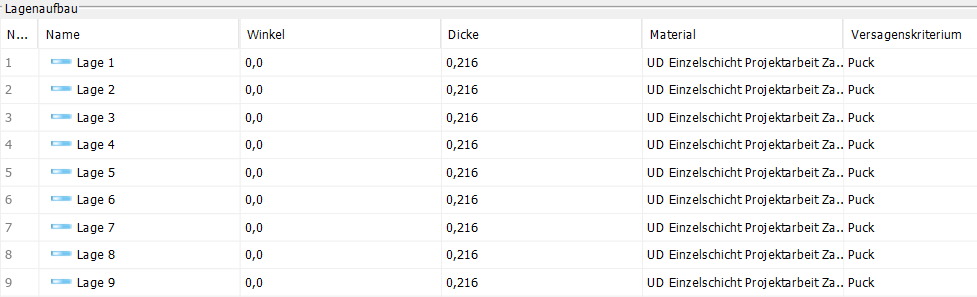
\includegraphics[width=1.0\textwidth]{Bilder/Lagenaufbau Holmgurte.png}
	\caption{Lagenaufbau Holmgurte}
	\label{fig:Lagenaufbau Holmgurte}
\end{figure}
\begin{figure}[h]
	\includegraphics[width=1.0\textwidth]{Bilder/Lagenaufbau Steg dünn.png}
	\caption{Lagenaufbau Steg Bereich $III$}
	\label{fig:Lagenaufbau Steg dünn}
\end{figure}
\begin{figure}[h]
	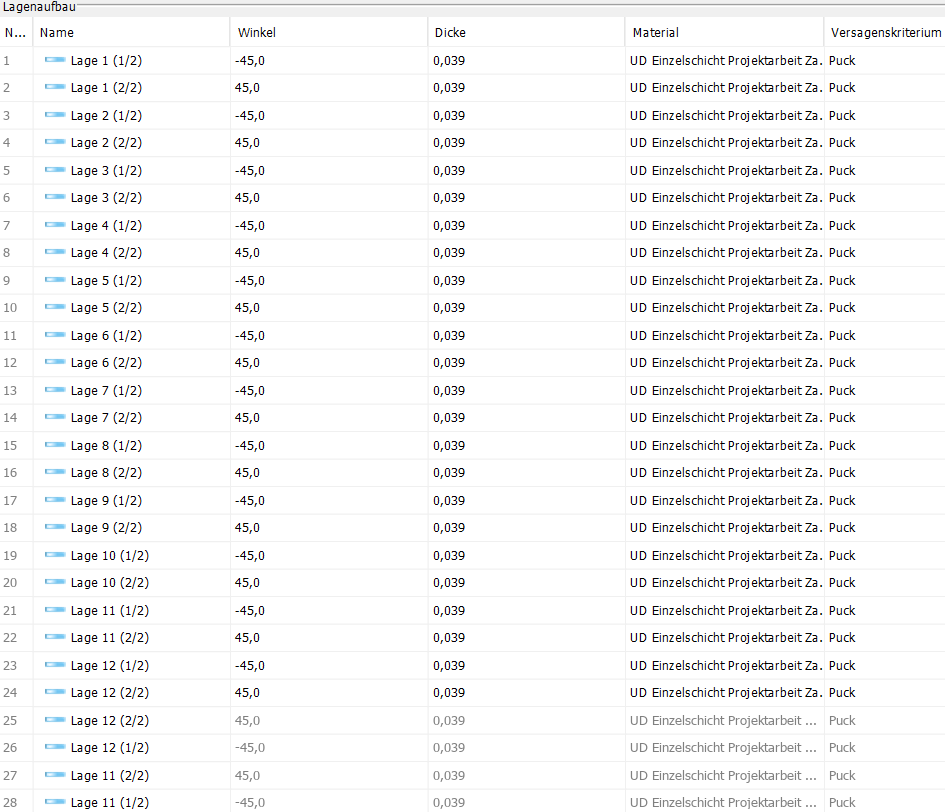
\includegraphics[width=1.0\textwidth]{Bilder/Lagenaufbau Steg dick.png}
	\caption{Lagenaufbau Steg Bereich $I$\&$II$}
	\label{fig:Lagenaufbau Steg dick}
\end{figure}
\begin{figure}[h]
	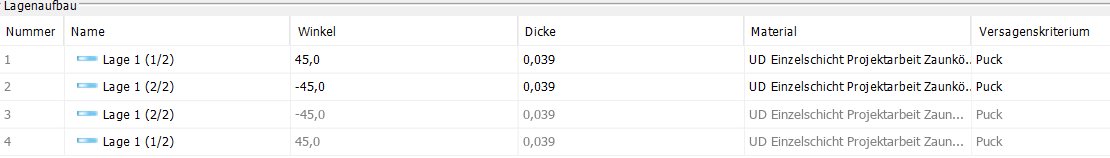
\includegraphics[width=1.0\textwidth]{Bilder/Lagenaufbau Haut.png}
	\caption{Lagenaufbau Flügelschale}
	\label{fig:Lagenaufbau Haut}
\end{figure}
\begin{figure}[h]
	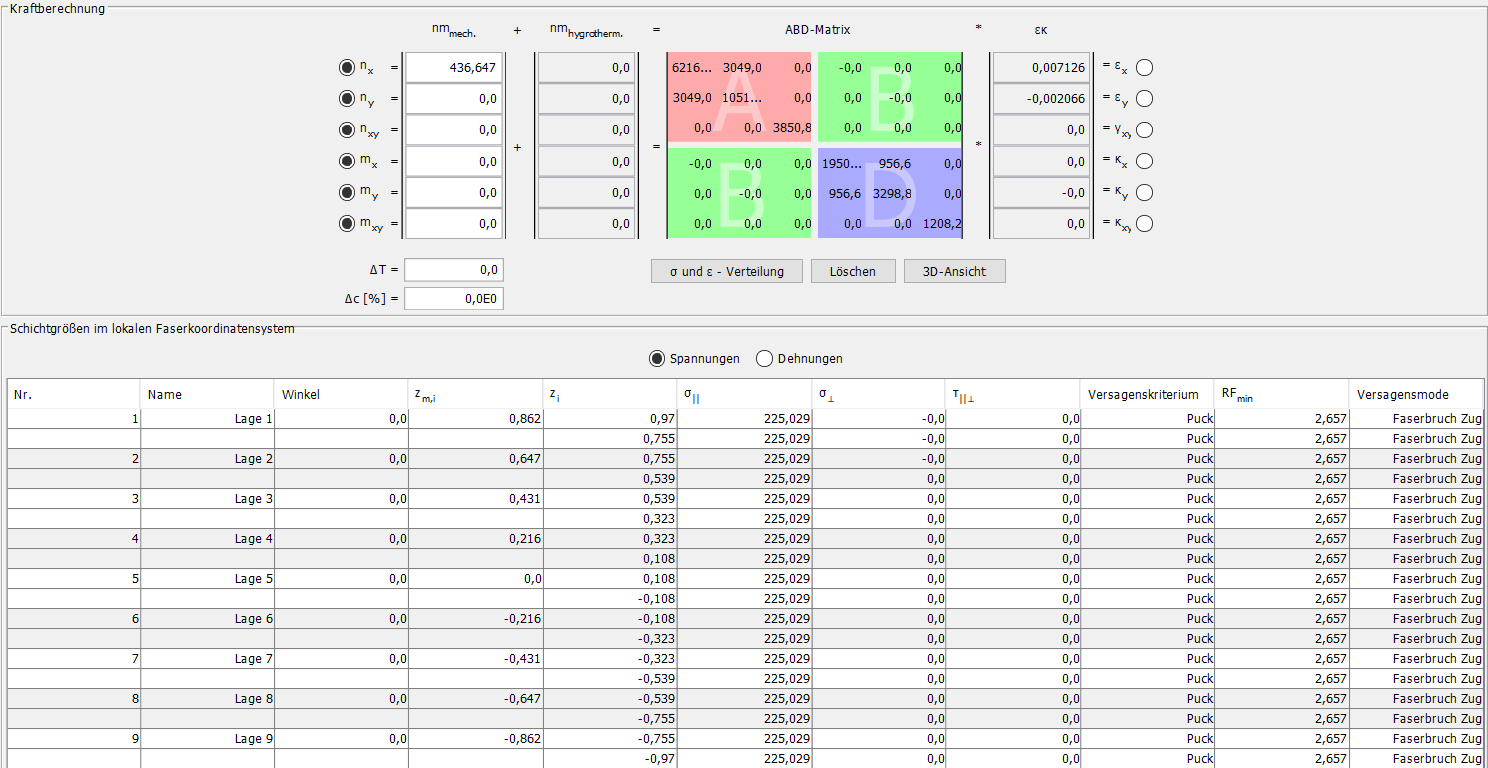
\includegraphics[width=1.0\textwidth]{Bilder/Berechnung Holmgurte.png}
	\caption{Berechnung Holmgurte}
	\label{fig:Berechnung Holmgurte}
\end{figure}
\begin{figure}[h]
	\includegraphics[width=1.0\textwidth]{Bilder/Berechnung Steg dünn.png}
	\caption{Berechnung Steg Bereich $III$}
	\label{fig:Berechnung Steg dünn}
\end{figure}
\begin{figure}[h]
	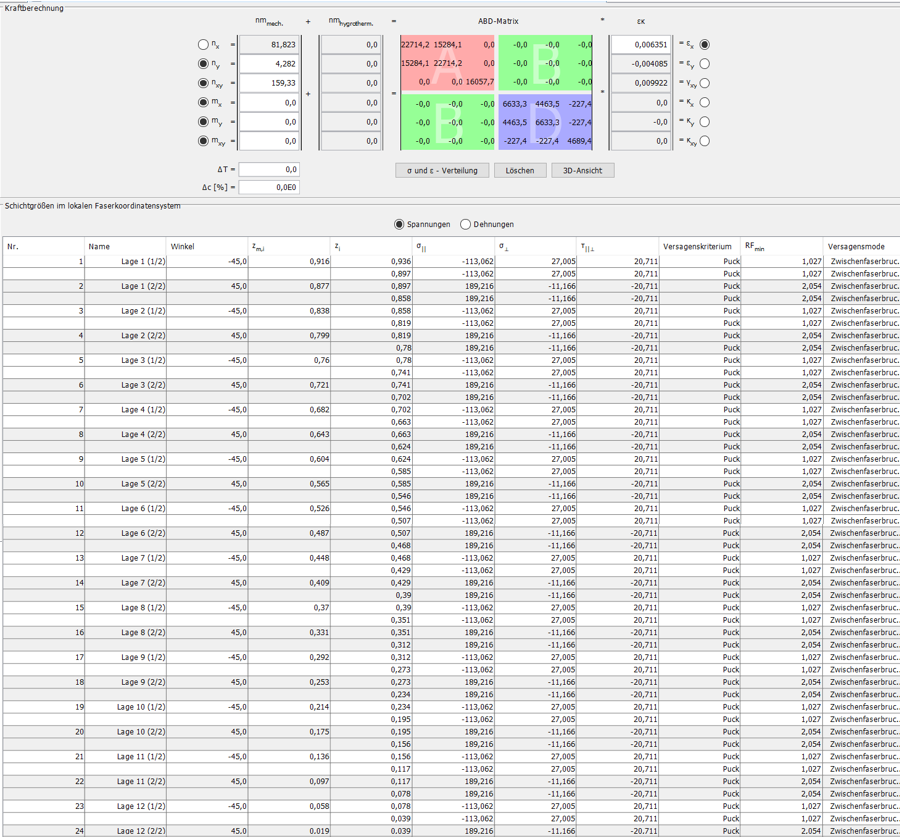
\includegraphics[width=1.0\textwidth]{Bilder/Berechnung Steg dick.png}
	\caption{Berechnung Steg Bereich $I$\&$II$}
	\label{fig:Berechnung Steg dick}
\end{figure}
\begin{figure}[h]
	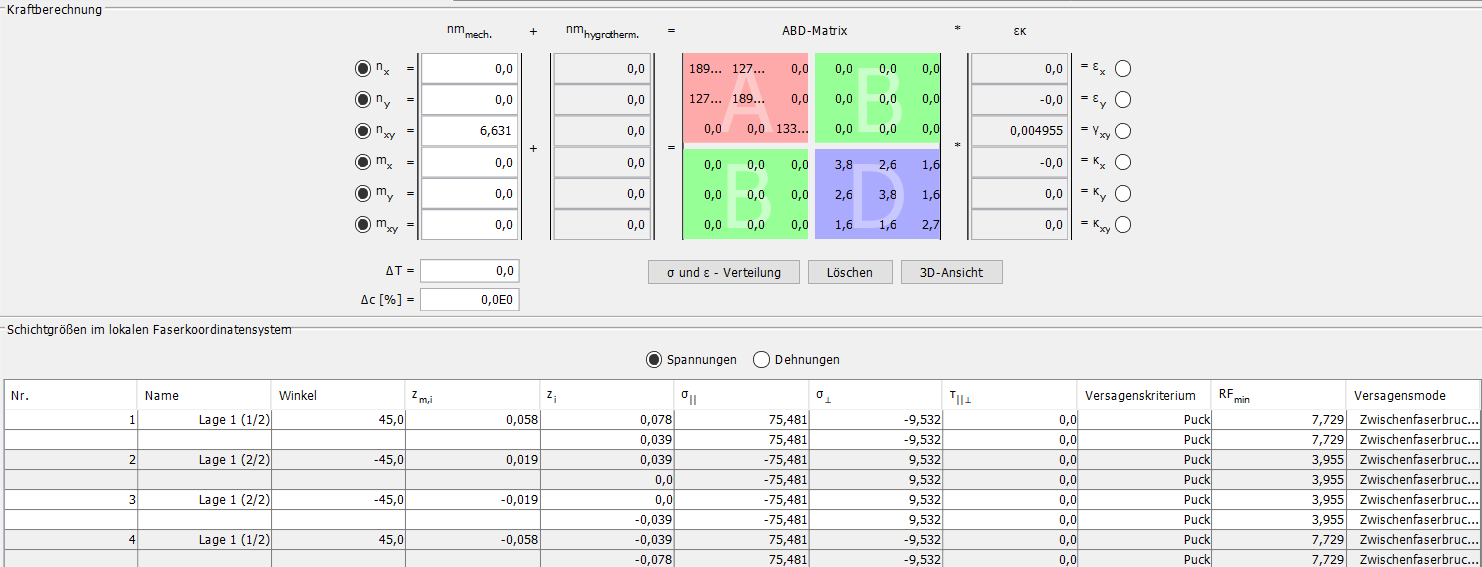
\includegraphics[width=1.0\textwidth]{Bilder/Berechnung Haut.png}
	\caption{Berechnung Flügelschale}
	\label{fig:Berechnung Haut}
\end{figure}
\begin{figure}[h]
	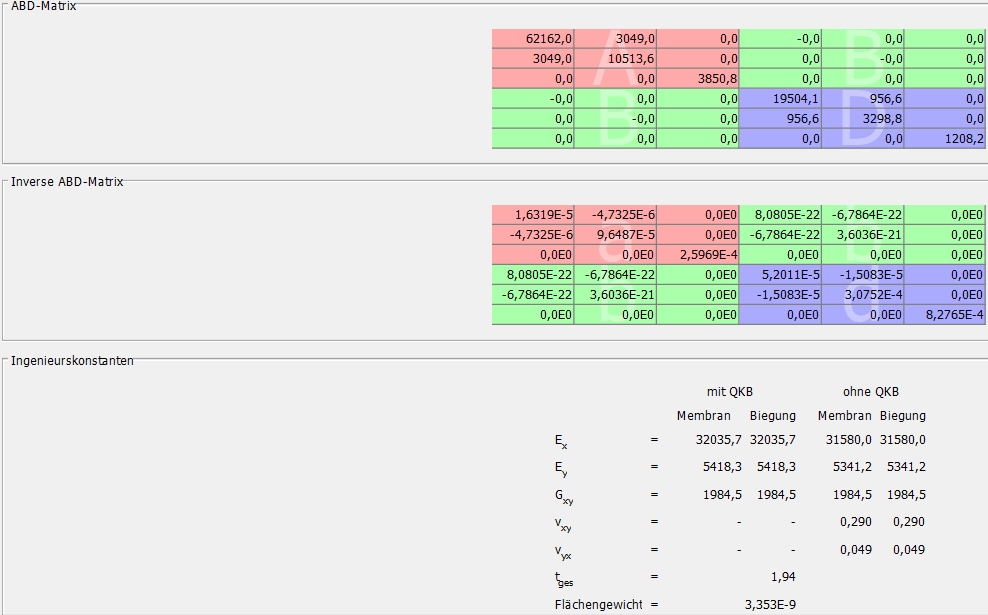
\includegraphics[width=1.0\textwidth]{Bilder/Konstanten Holmgurte.png}
	\caption{Ingenieurskonstanten Holmgurte}
	\label{fig:Ingenieurskonstanten Holmgurte}
\end{figure}
\begin{figure}[h]
	\includegraphics[width=1.0\textwidth]{Bilder/Konstanten Steg dünn.png}
	\caption{BerechnIngenieurskonstantenung Steg Bereich $III$}
	\label{fig:Ingenieurskonstanten Steg dünn}
\end{figure}
\begin{figure}[h]
	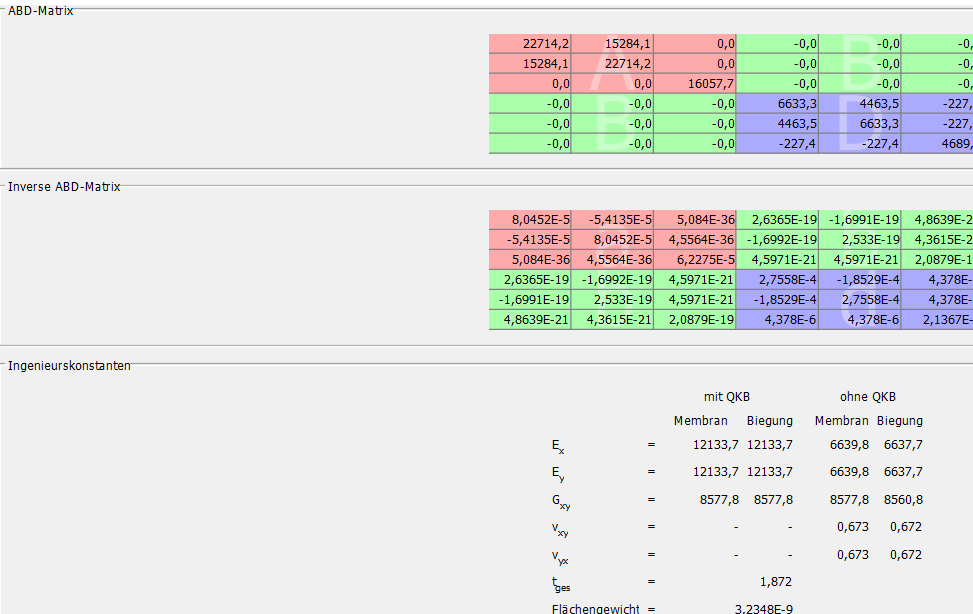
\includegraphics[width=1.0\textwidth]{Bilder/Konstanten Steg dick.png}
	\caption{BerechnIngenieurskonstantenung Steg Bereich $I\&II$}
	\label{fig:Ingenieurskonstanten Steg dick}
\end{figure}
\begin{figure}[h]
	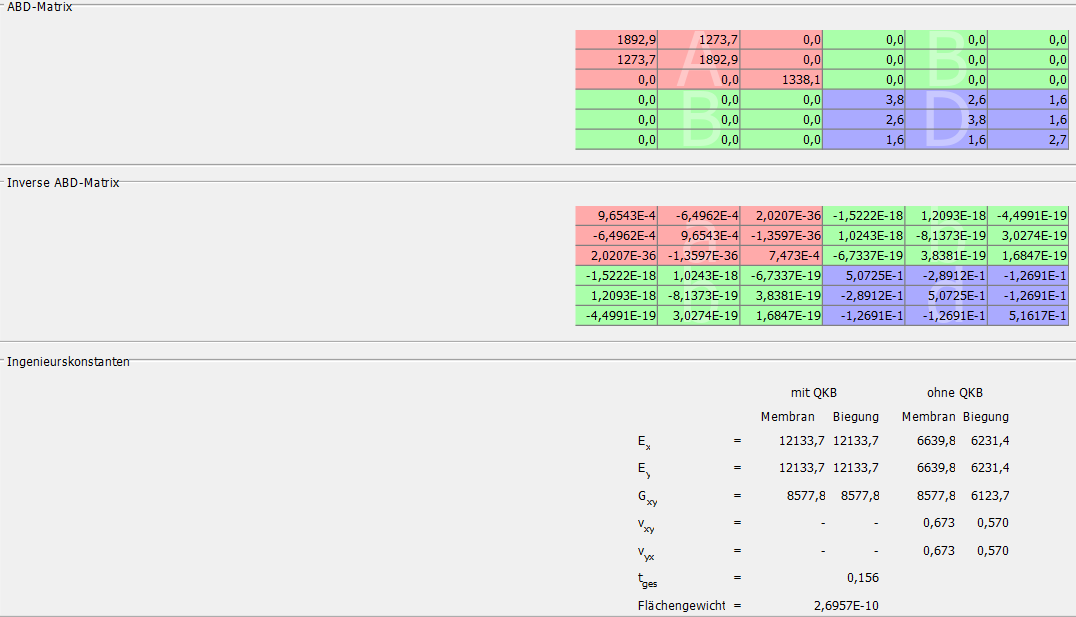
\includegraphics[width=1.0\textwidth]{Bilder/Konstanten Haut.png}
	\caption{Ingenieurskonstanten Flügelschale}
	\label{fig:Ingenieurskonstanten Haut}
\end{figure}
\begin{figure}[h]
	\centering
	\includegraphics[width=0.3\textwidth]{Bilder/Längen.png}
	\caption{Wertebereich der Laufvariablen $s_i$}
	\label{fig:LaengenS}
\end{figure}
\begin{figure}[h]
	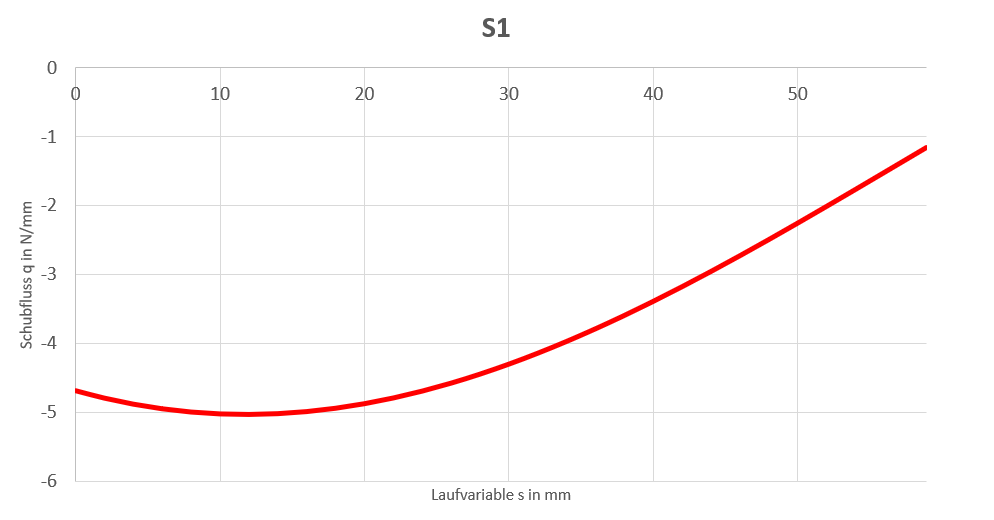
\includegraphics[width=1.0\textwidth]{Bilder/S1.png}
	\caption{Schubfluss Bereich 1}
	\label{fig:S1}
\end{figure}
\begin{figure}[h]
	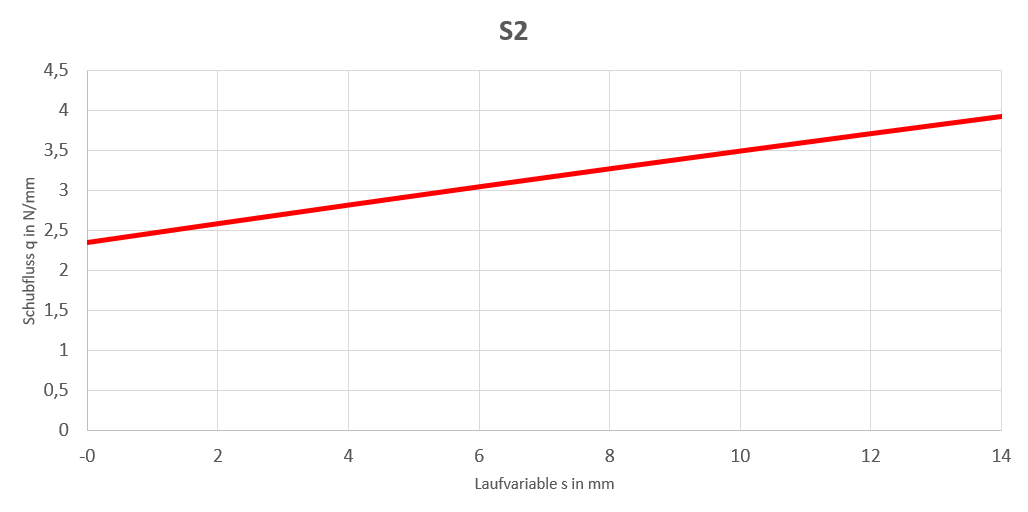
\includegraphics[width=1.0\textwidth]{Bilder/S2.png}
	\caption{Schubfluss Bereich 2}
\end{figure}
\begin{figure}[h]
	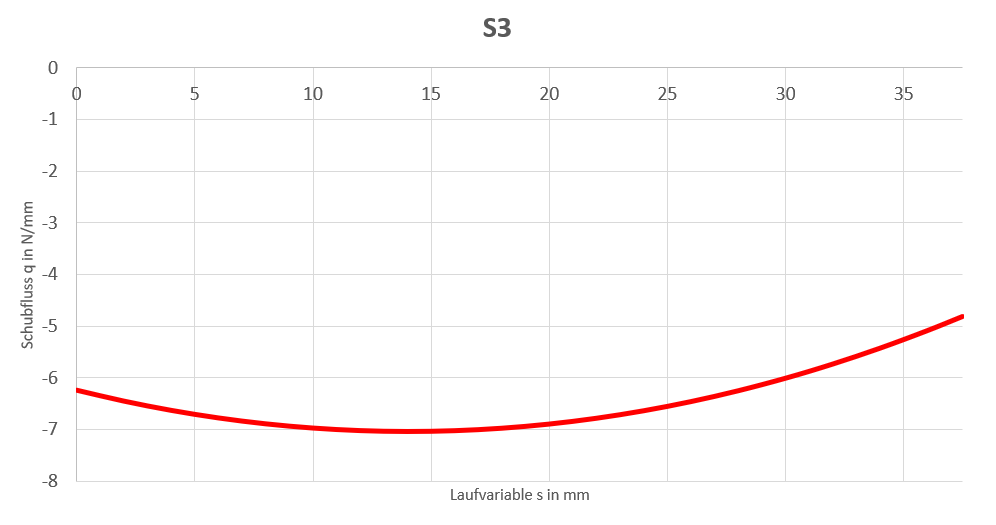
\includegraphics[width=1.0\textwidth]{Bilder/S3.png}
	\caption{Schubfluss Bereich 3}
\end{figure}
\begin{figure}[h]
	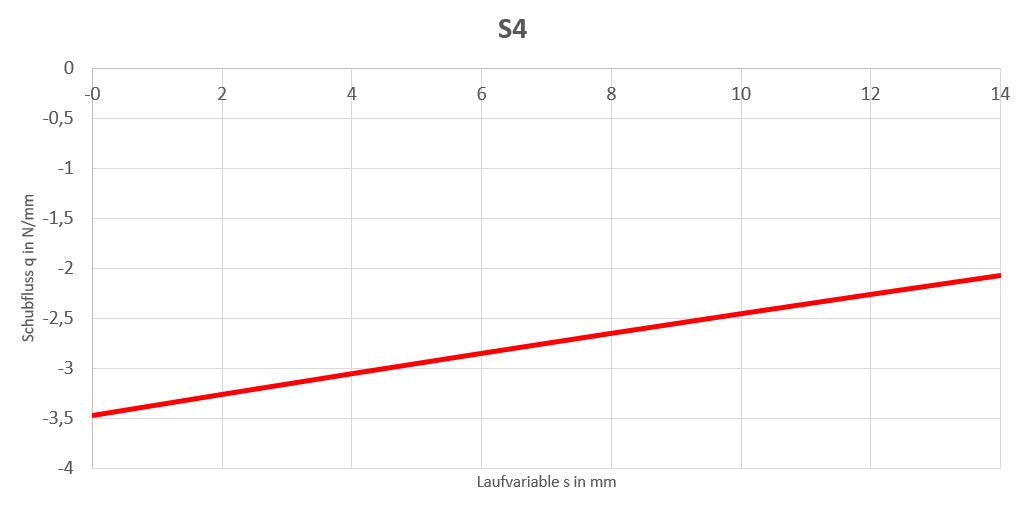
\includegraphics[width=1.0\textwidth]{Bilder/S4.png}
	\caption{Schubfluss Bereich 4}
	\label{fig:S4}
\end{figure}
\begin{figure}[h]
	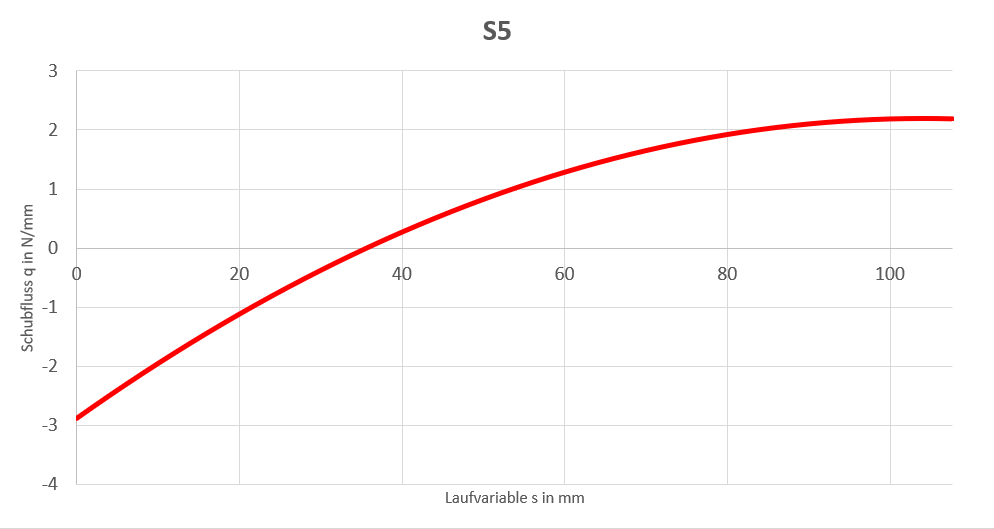
\includegraphics[width=1.0\textwidth]{Bilder/S5.png}
	\caption{Schubfluss Bereich 5}
\end{figure}
\begin{figure}[h]
	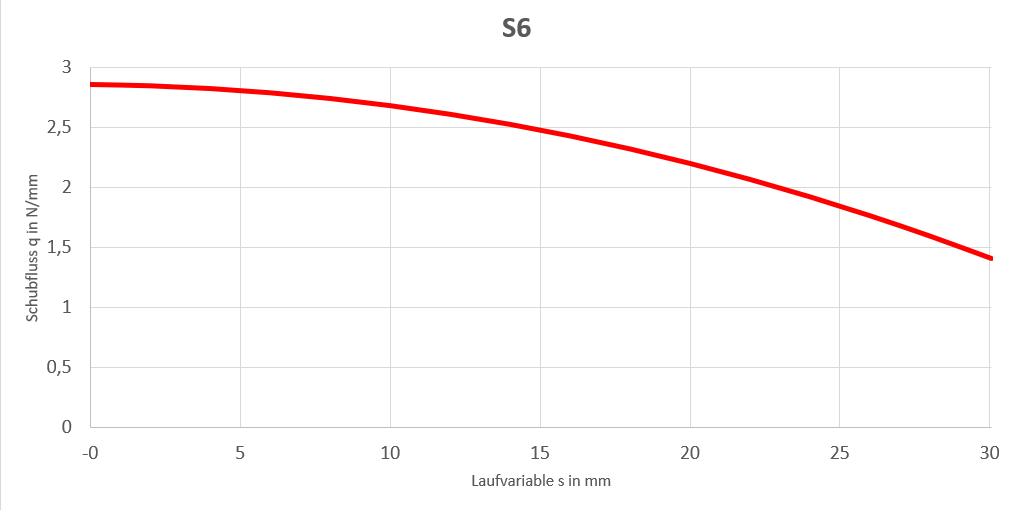
\includegraphics[width=1.0\textwidth]{Bilder/S6.png}
	\caption{Schubfluss Bereich 6}
\end{figure}
\begin{figure}[h]
	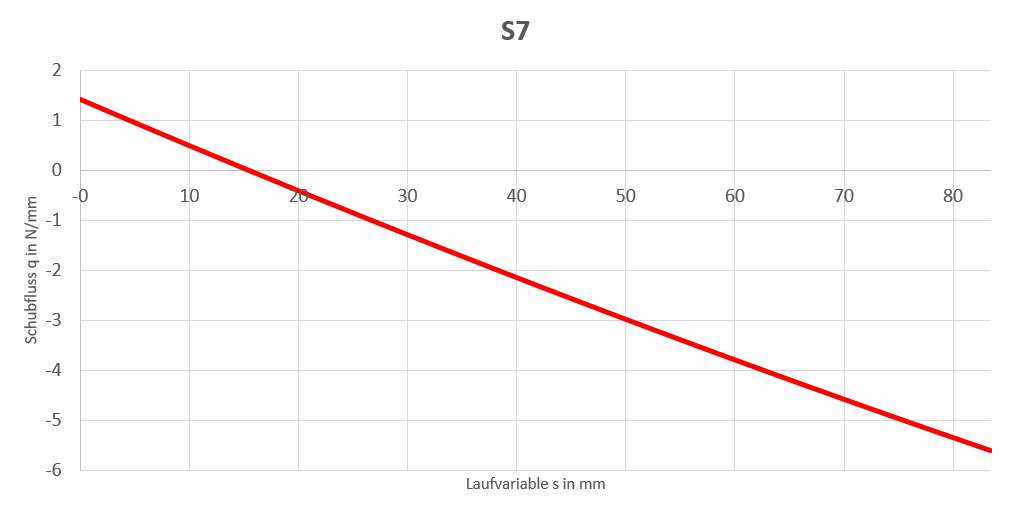
\includegraphics[width=1.0\textwidth]{Bilder/S7.png}
	\caption{Schubfluss Bereich 7}
\end{figure}
\begin{figure}[h]
	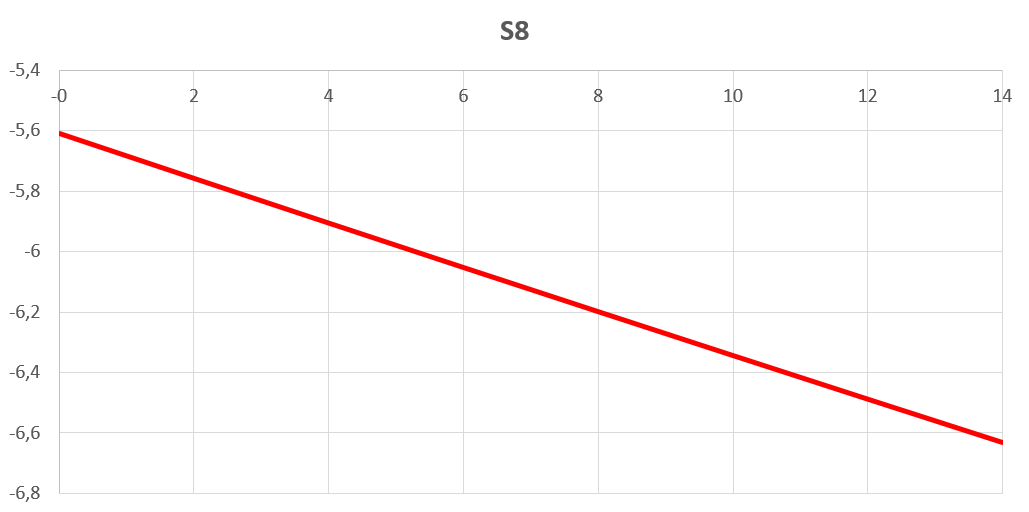
\includegraphics[width=1.0\textwidth]{Bilder/S8.png}
	\caption{Schubfluss Bereich 8}
\end{figure}
\begin{figure}[h]
	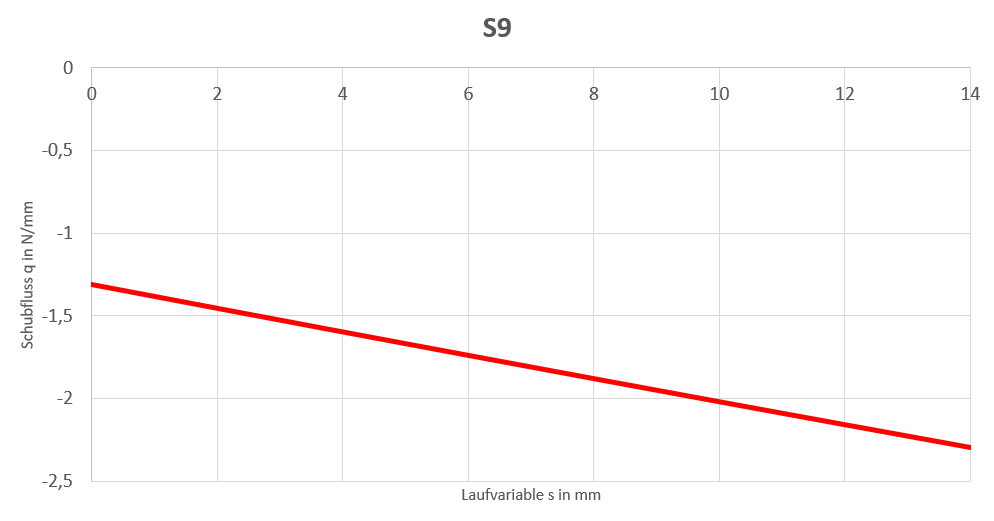
\includegraphics[width=1.0\textwidth]{Bilder/S9.png}
	\caption{Schubfluss Bereich 9}
\end{figure}
\begin{figure}[h]
	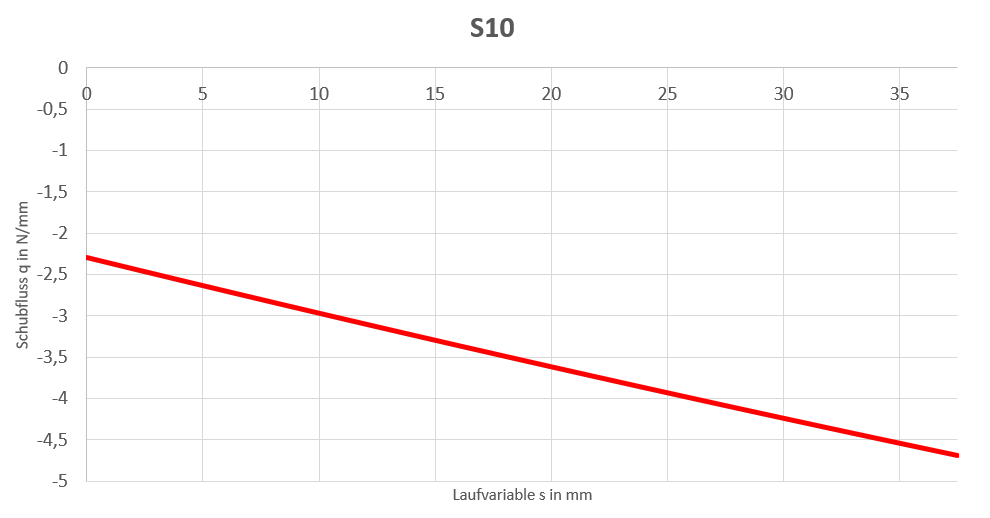
\includegraphics[width=1.0\textwidth]{Bilder/S10.png}
	\caption{Schubfluss Bereich 10}
	\label{fig:S10}
\end{figure}
\newpage
%Technische Zeichnungen
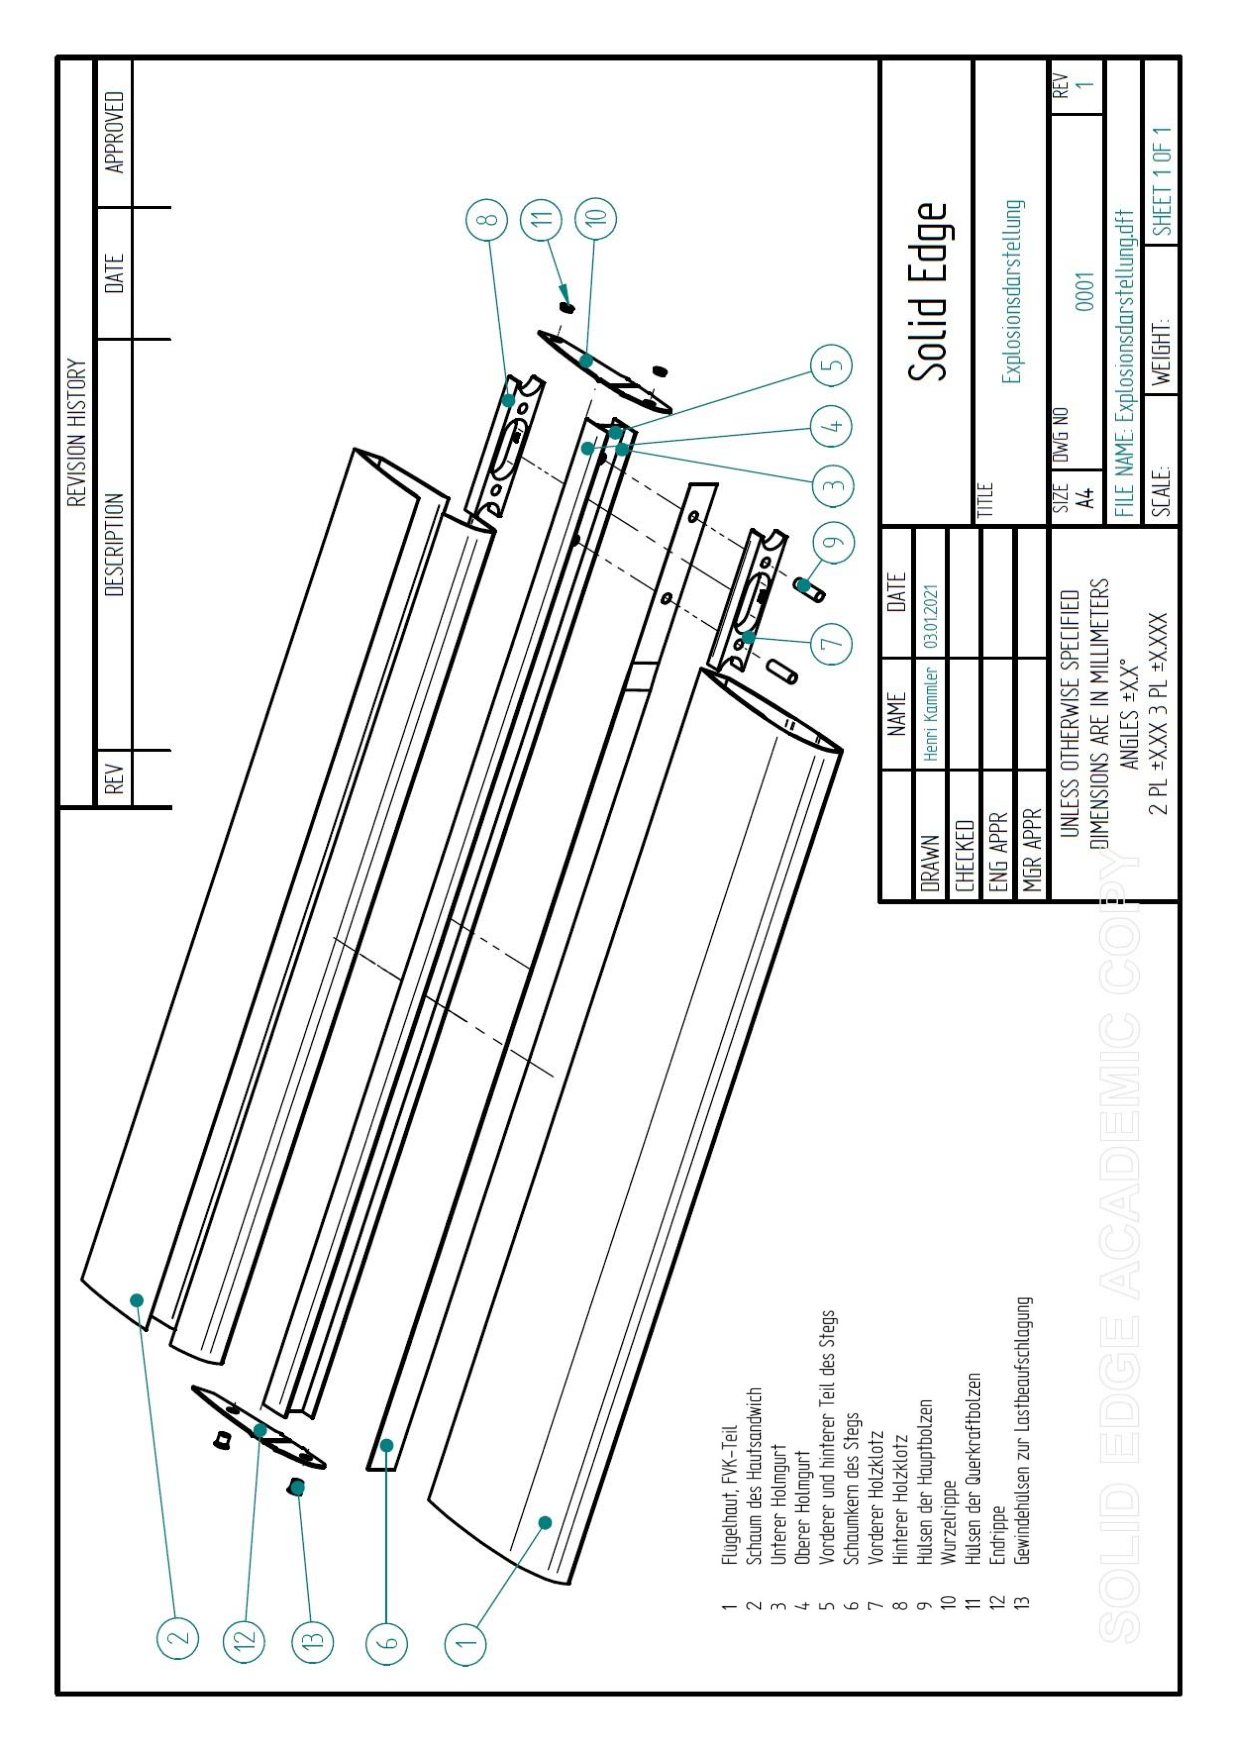
\includepdf[pages=-]{PDFs/ExplosionConvBez.pdf}
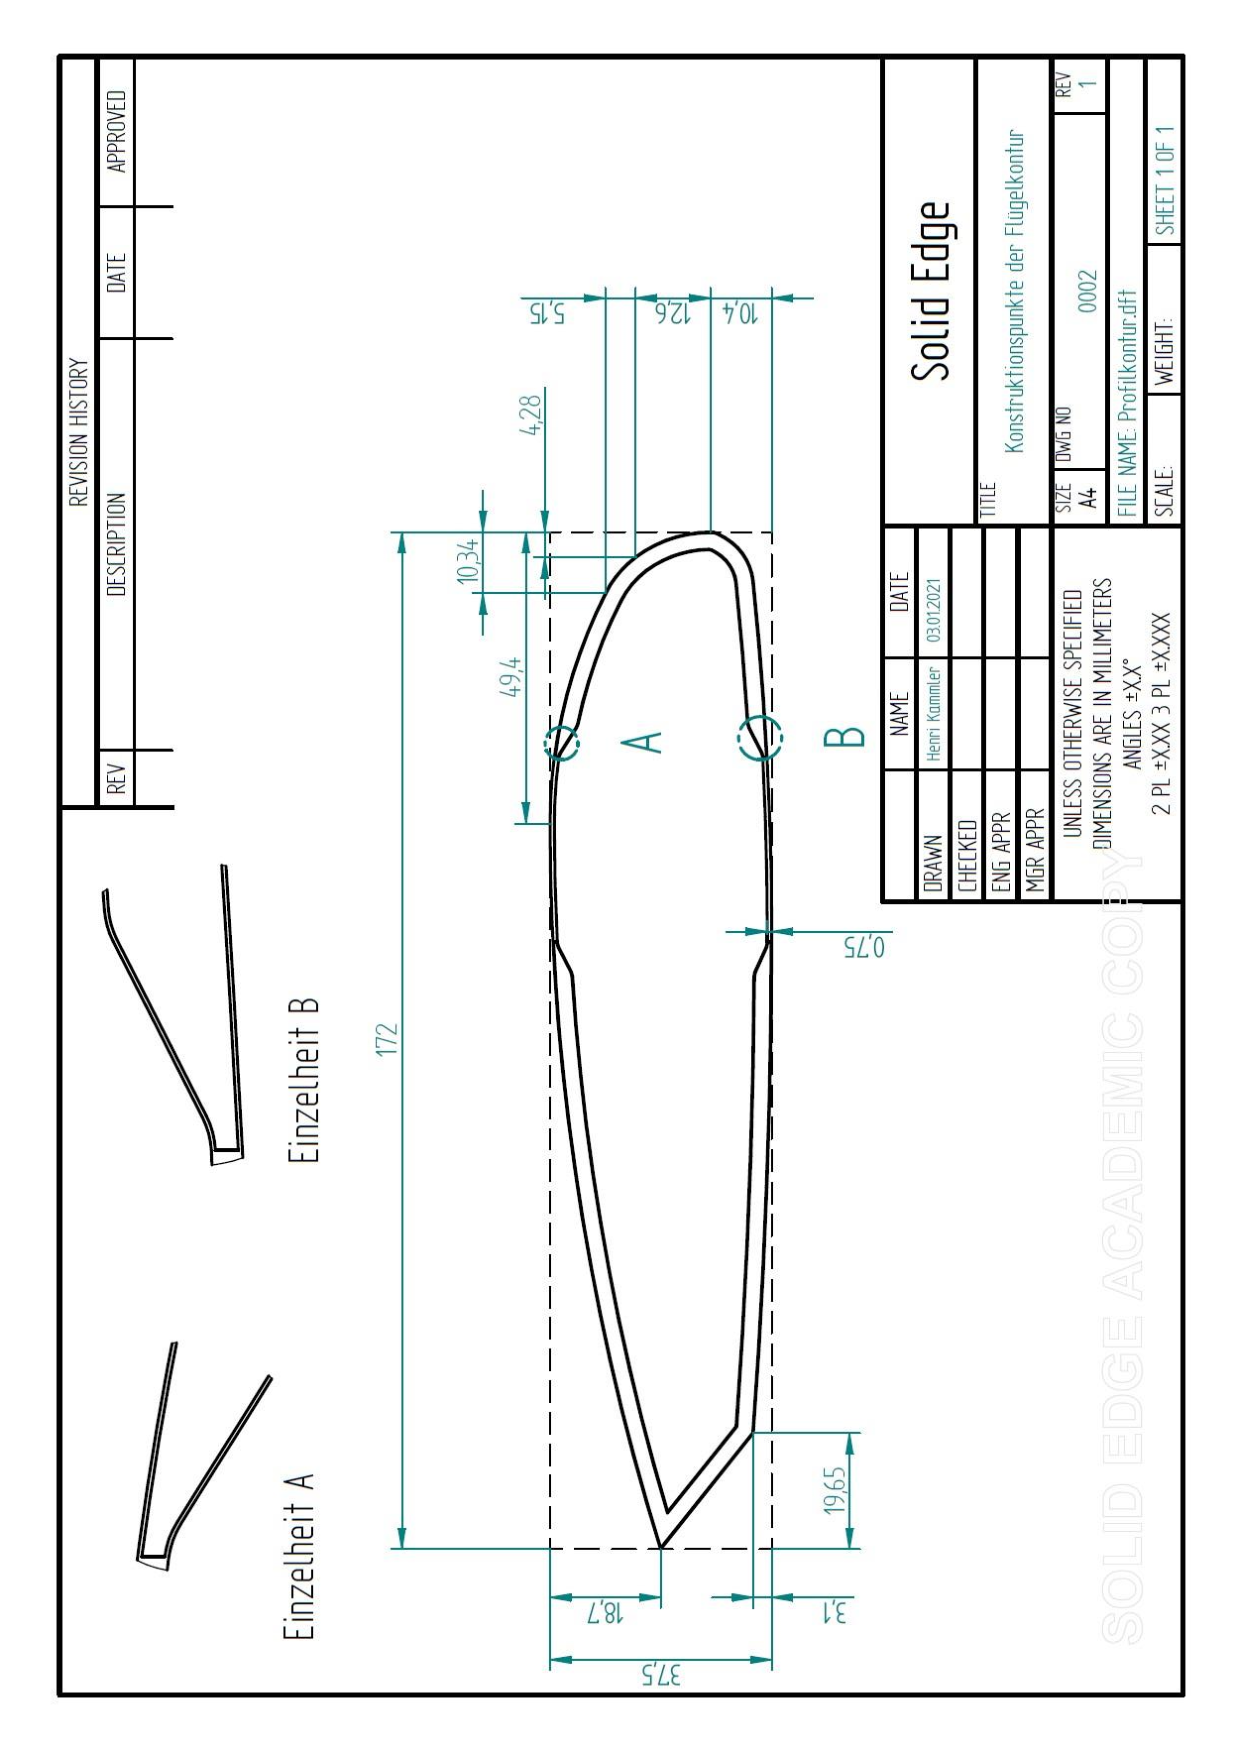
\includepdf[pages=-]{PDFs/ProfilkonturConv.pdf}
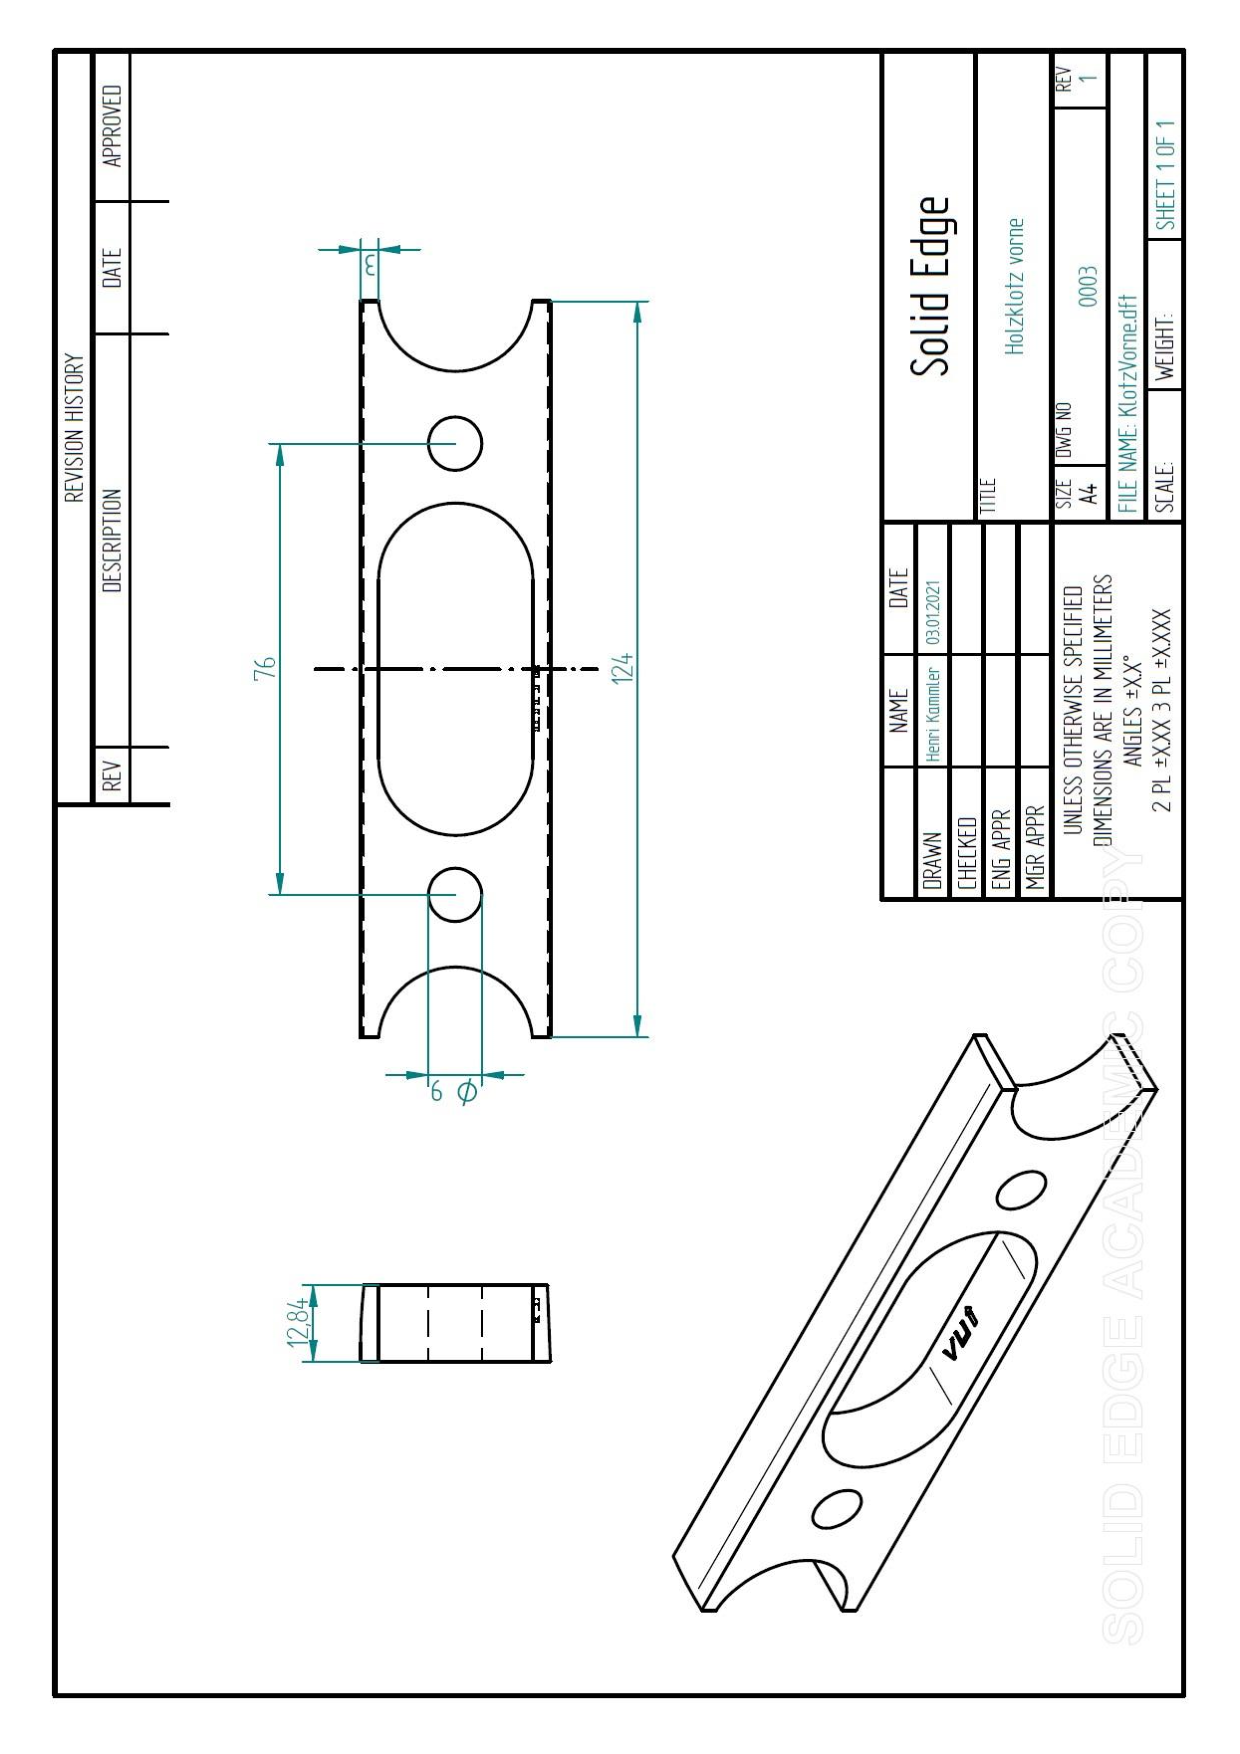
\includepdf[pages=-]{PDFs/KlotzVorne.pdf}
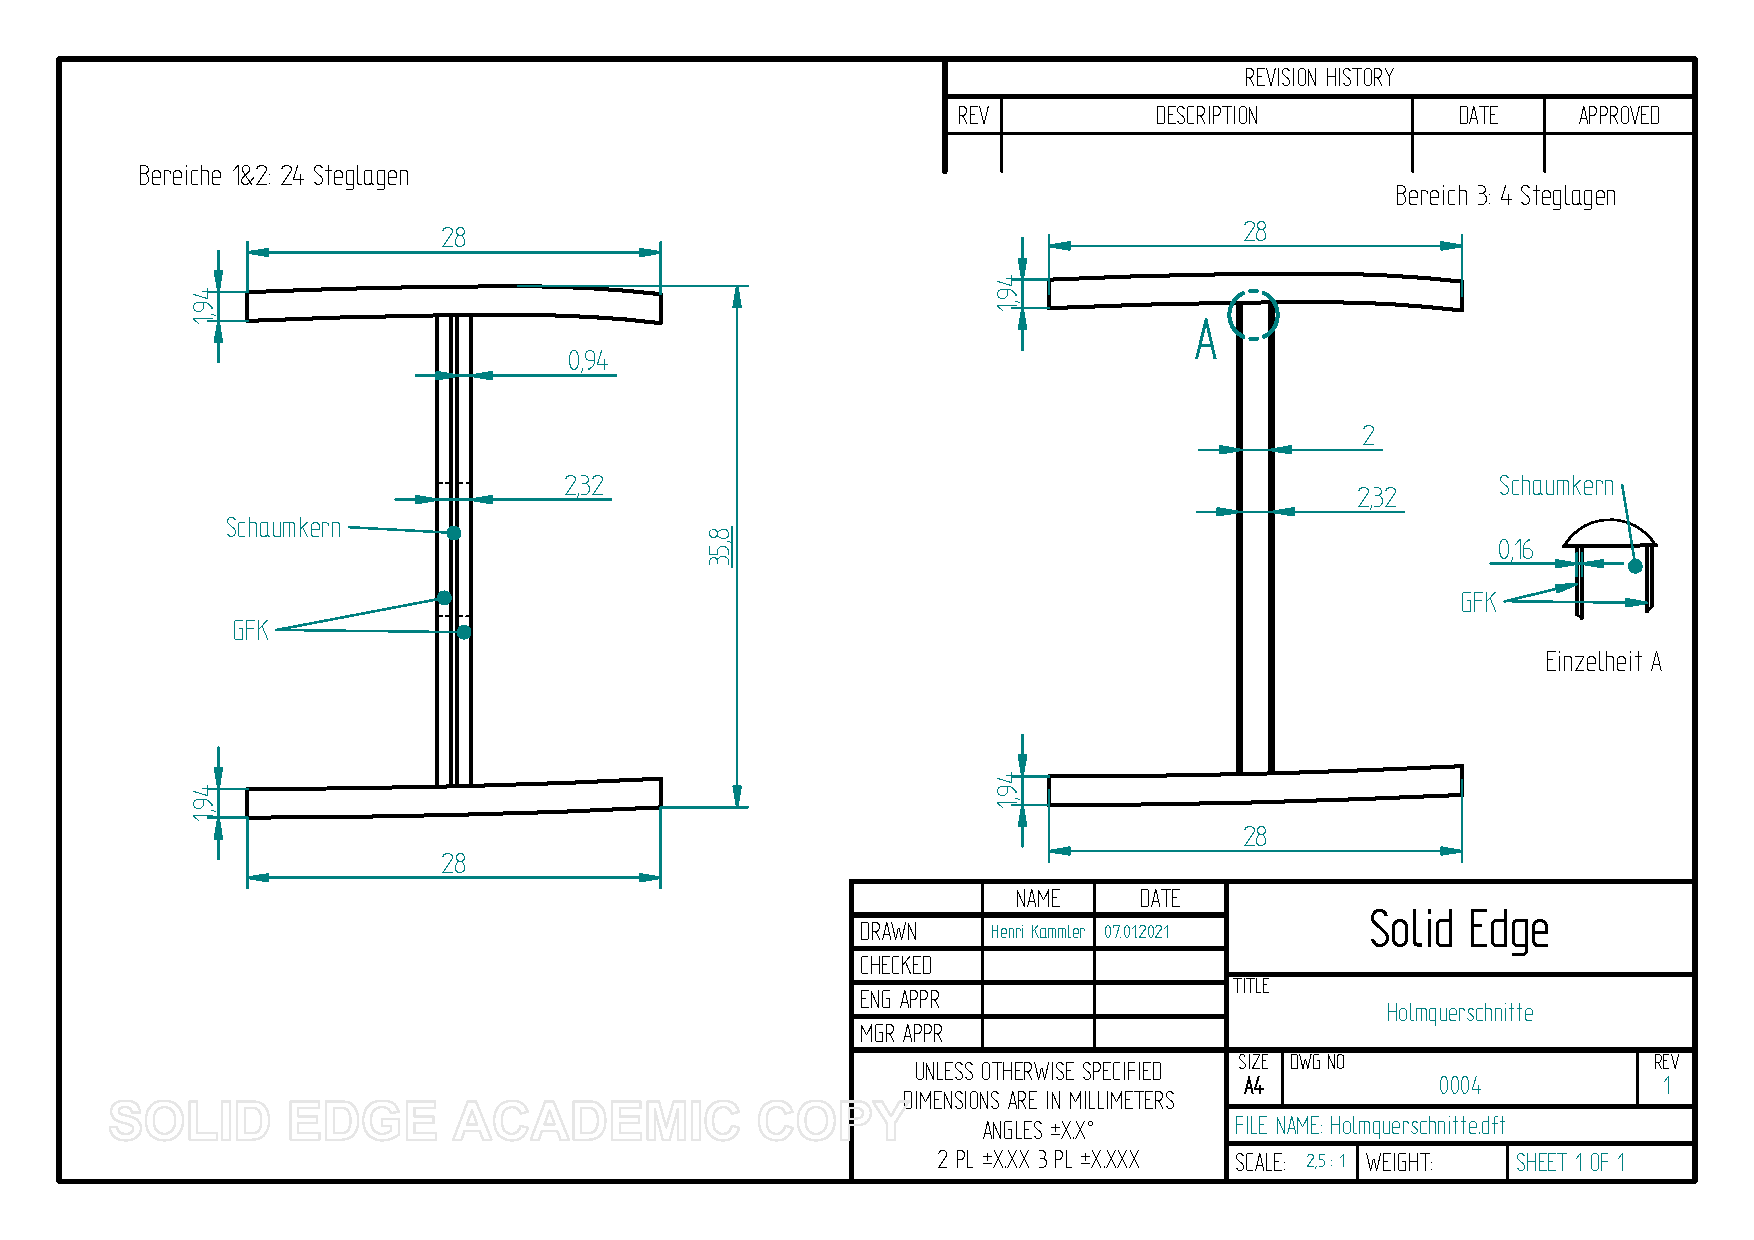
\includepdf[pages=-]{PDFs/Holmquerschnitte.pdf}

\begin{figure}[h]
	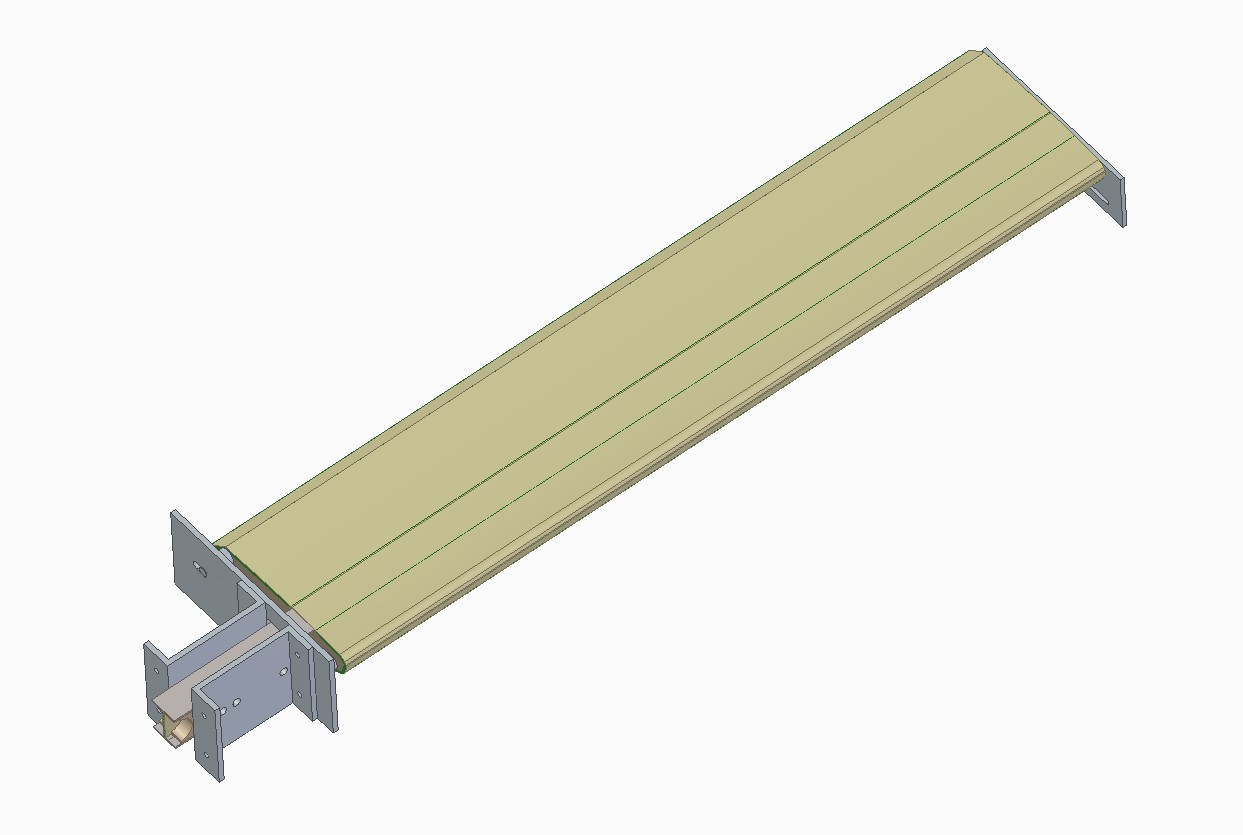
\includegraphics[width=1.0\textwidth]{Bilder/AufbauGesamt.jpg}
	\caption{CAD-Modell der Tragfläche und des Teststandes}
	\label{fig:AufbauGesamt}
\end{figure}

\begin{figure}[h]
	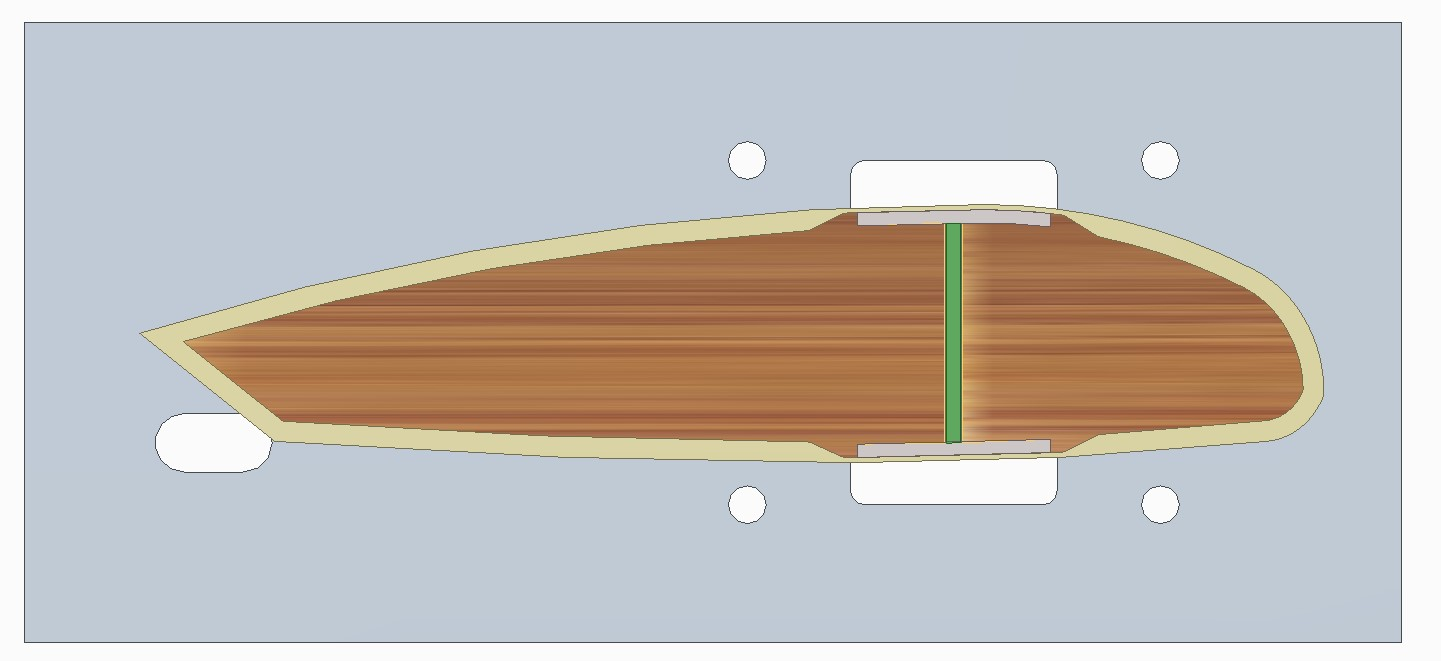
\includegraphics[width=1.0\textwidth]{Bilder/SeiteRichtig.jpg}
	\caption{Ursprüngliche Lage des hinteren Langlochs der Querkraftbolzen}
	\label{fig: SeiteRichtig}
\end{figure}

\begin{figure}[h]
	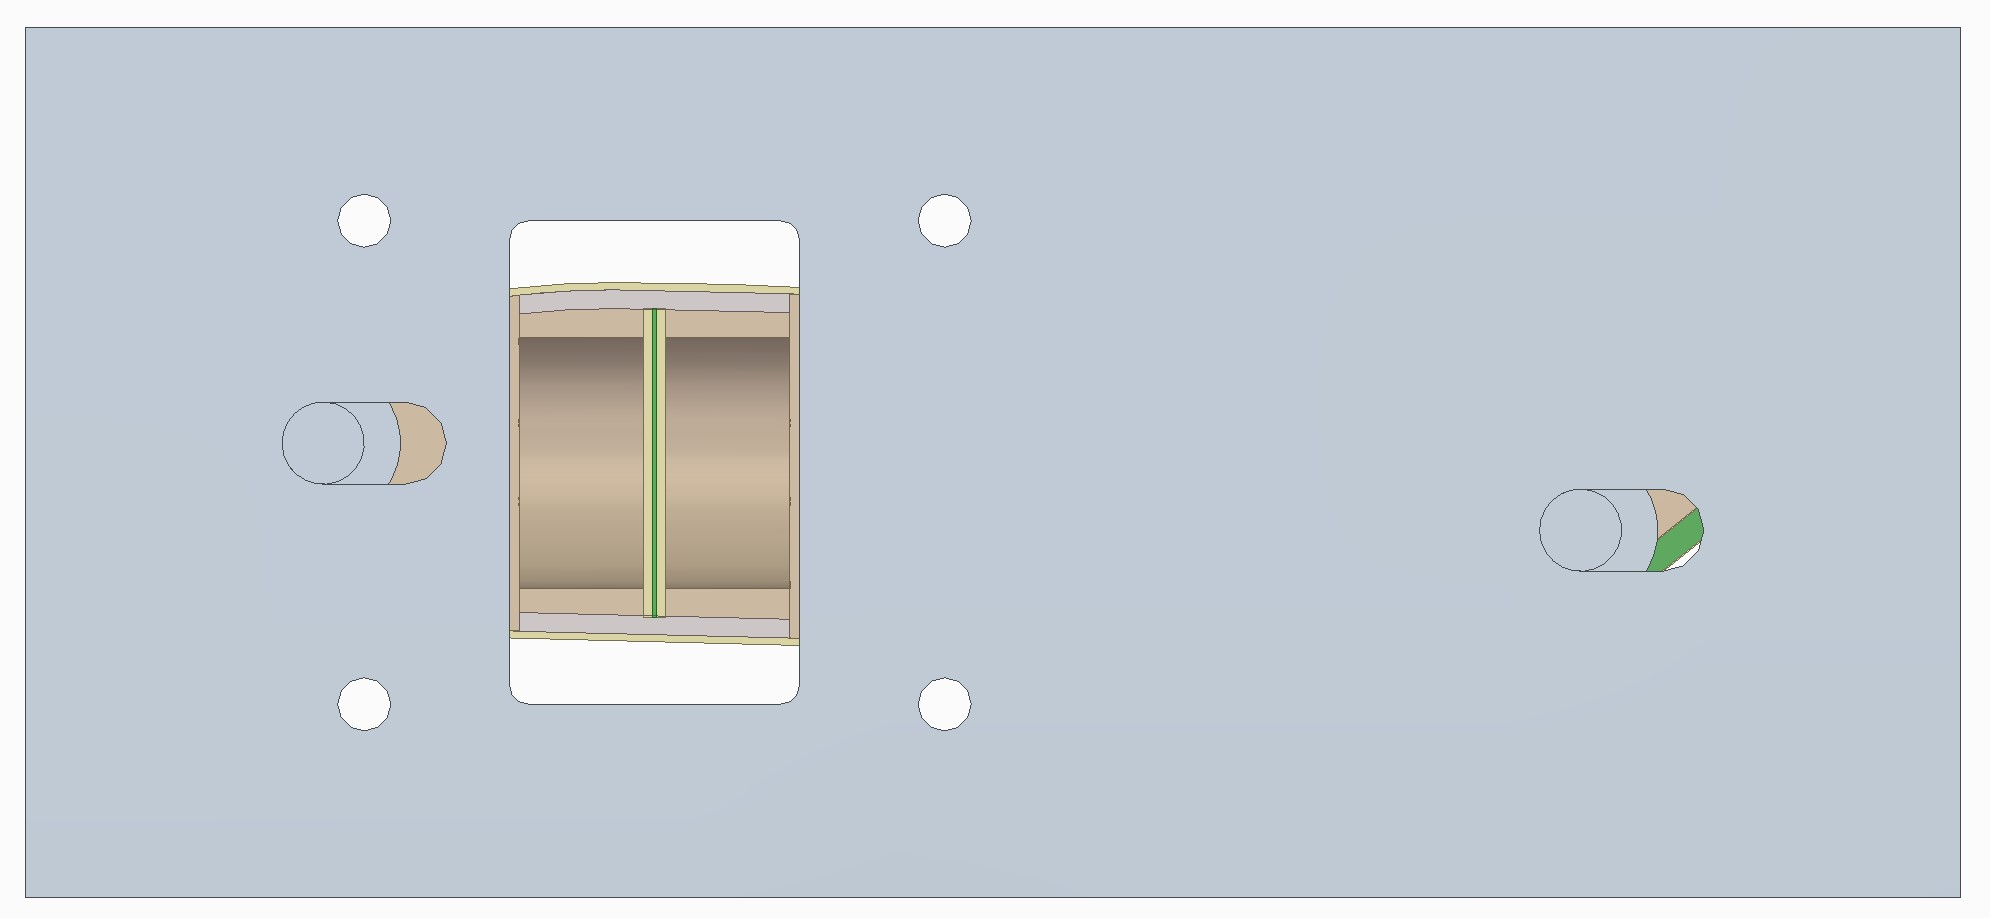
\includegraphics[width=1.0\textwidth]{Bilder/MontagePlatte.jpg}
	\caption{Montage der Tragfläche auf dem Teststand}
	\label{fig:MontagePlatte}
\end{figure}
\begin{figure}[h]
 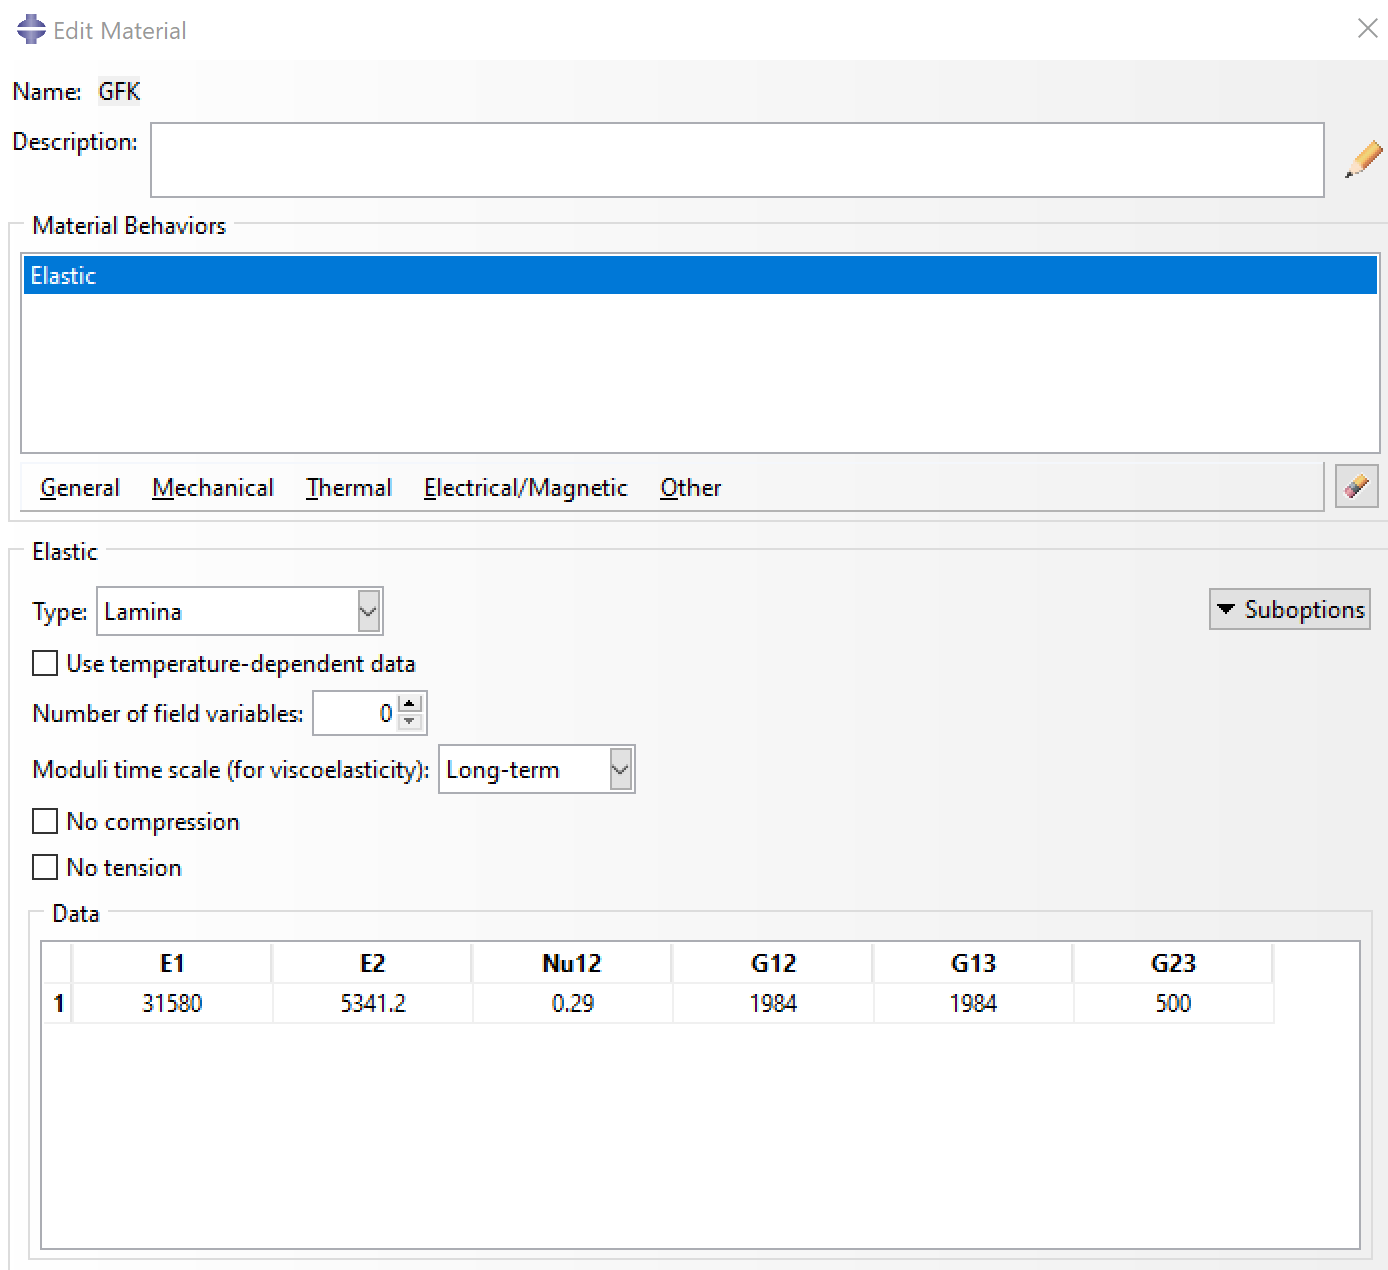
\includegraphics[width=0.8\textwidth]{Bilder/Material_GFK}
 \caption{ABAQUS Material Beispiel GFK}
 \label{Material}
\end{figure}
\begin{figure}[h]
\centering
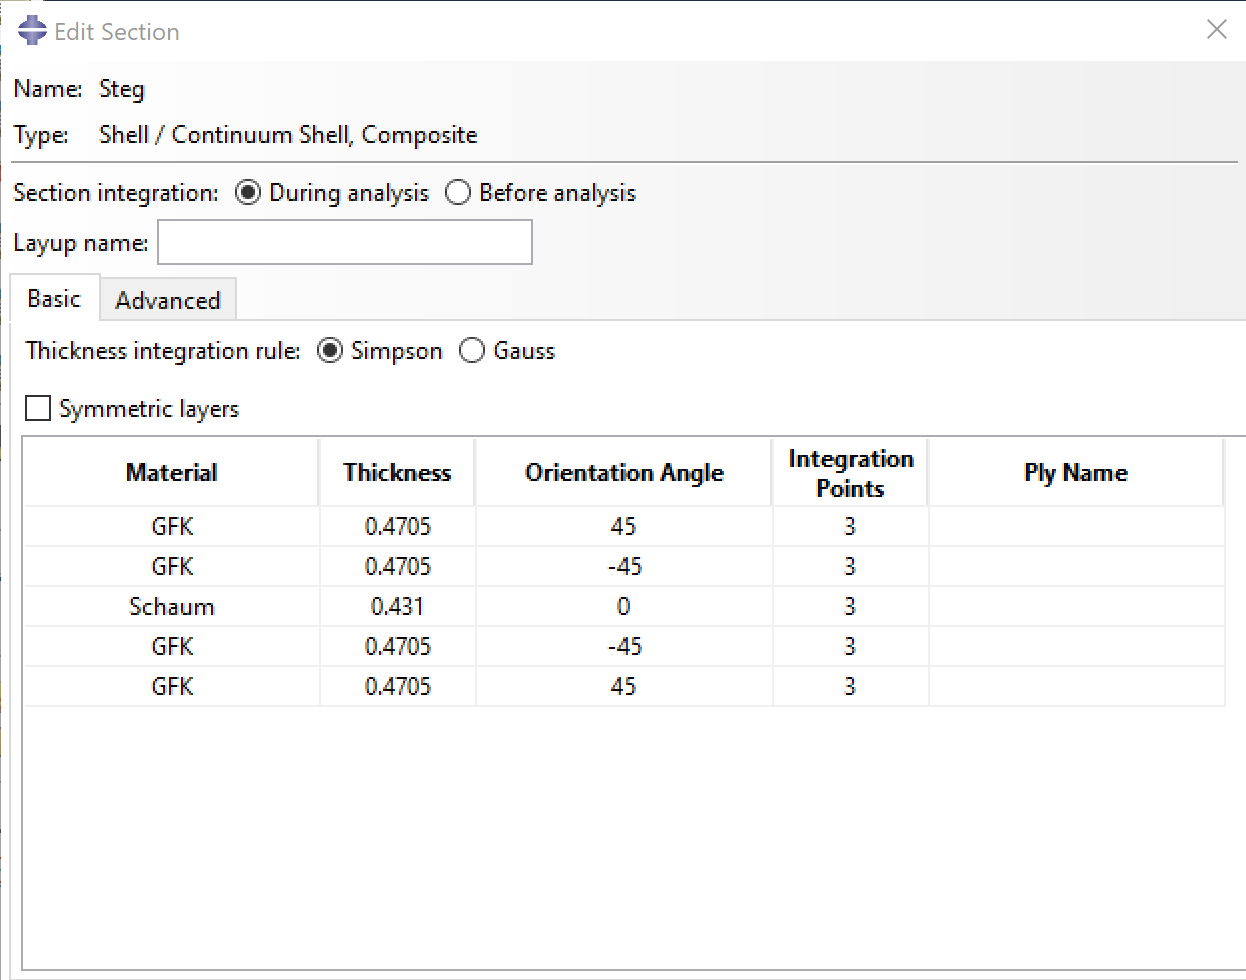
\includegraphics[width=0.8\textwidth]{Bilder/Steg_Material}
\label{Steg_Material}
\caption{ABAQUS Section Beispiel:Steg}
\end{figure}

\begin{figure}[h]
 \centering
 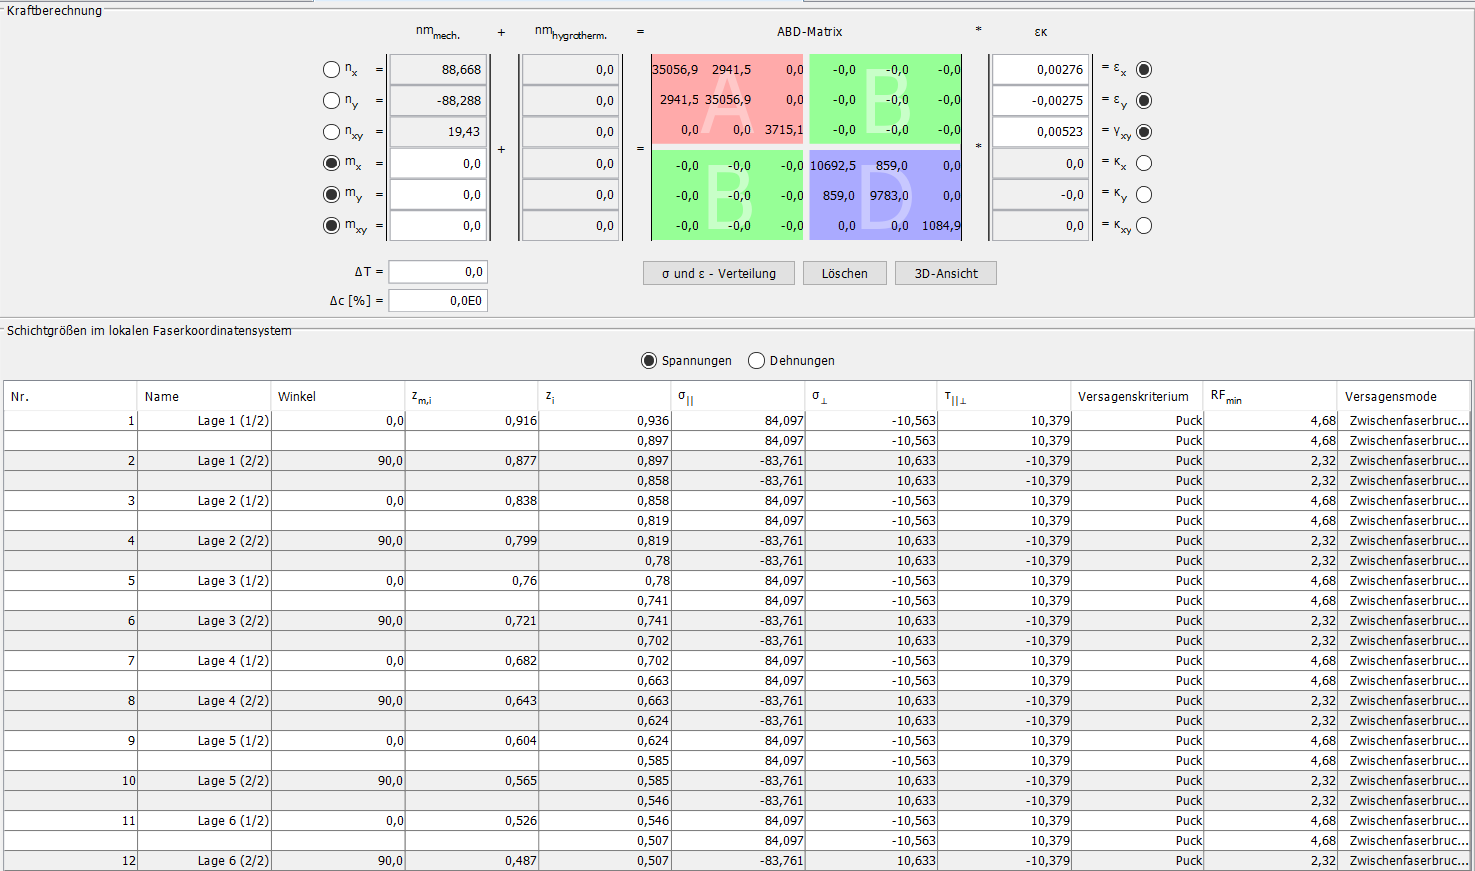
\includegraphics[width=1\textwidth]{Bilder/sicher1}
 \label{sicher-steg}
 \caption{Sicherheit im Steg bei 500N}
\end{figure}
\begin{figure}[h]
\centering
\includegraphics[width=1\textwidth]{Bilder/sicher2}
\caption{Sicherheit in der Haut bei 500N}
\end{figure}
\begin{figure}[h]
\centering
\includegraphics[width=1\textwidth]{Bilder/sicher3}
\caption{Sicherheit am Gurt oben bei 500N}
\end{figure}
\begin{figure}[h]
\centering
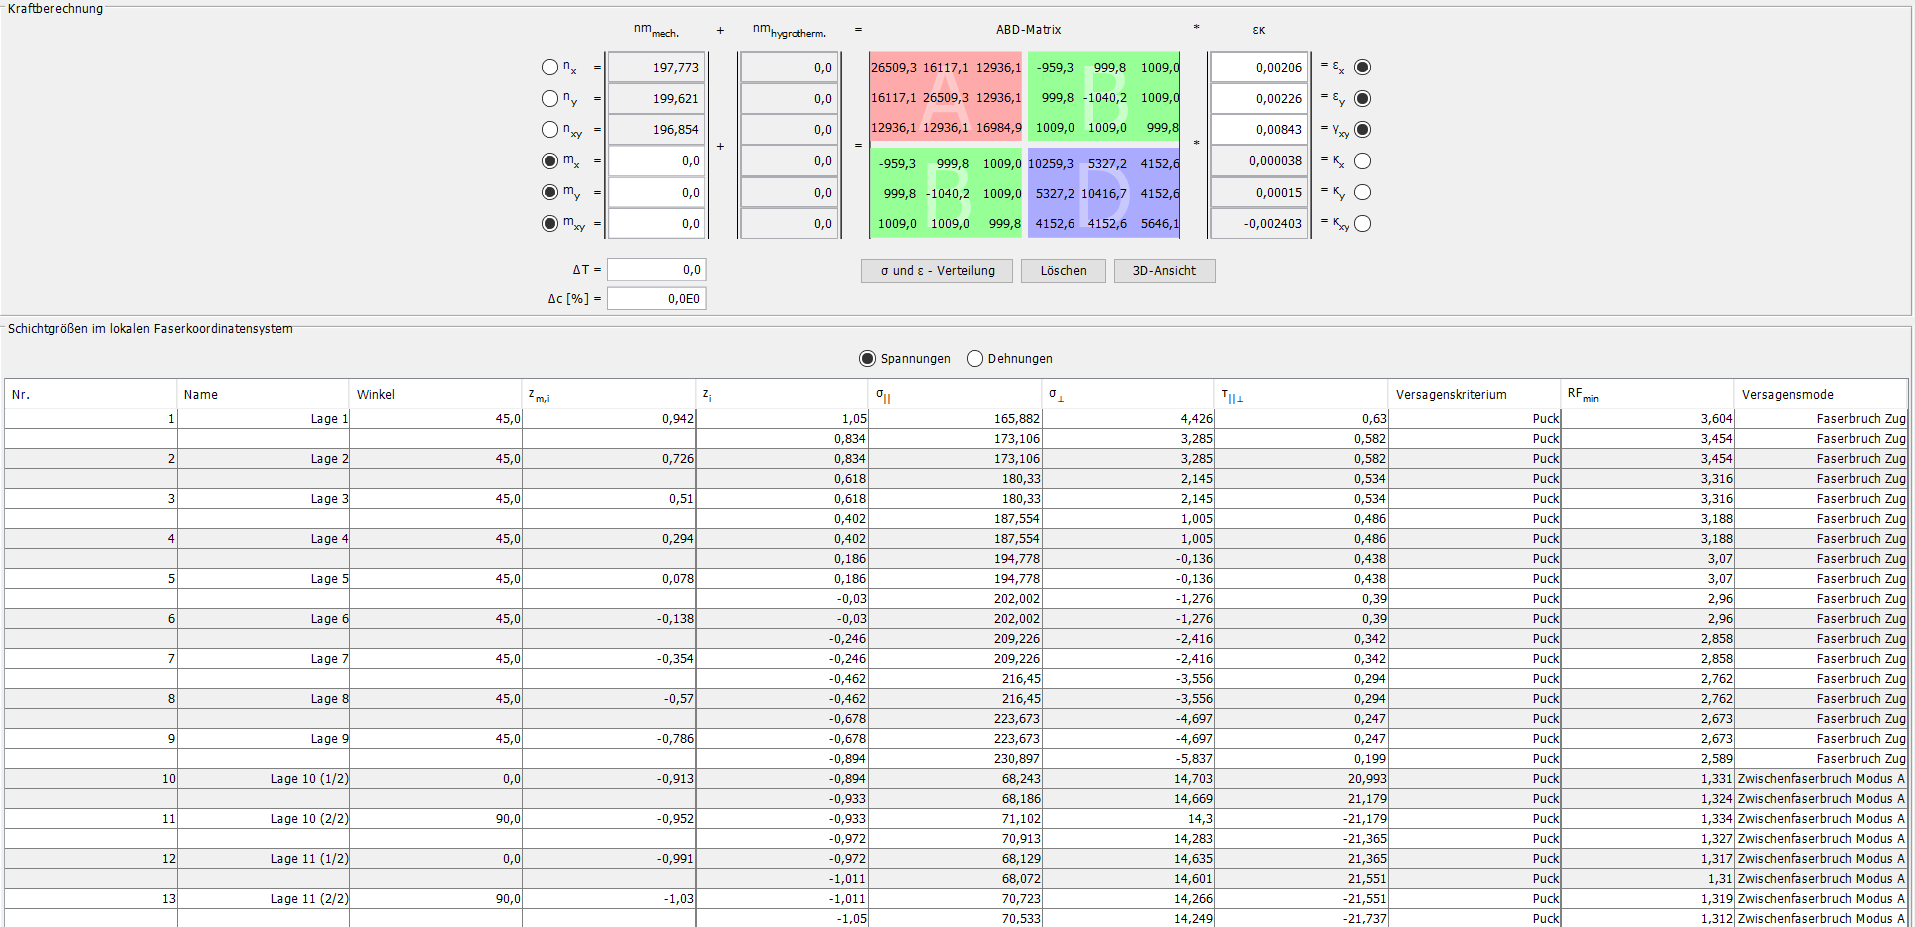
\includegraphics[width=1\textwidth]{Bilder/sicher4}
\label{sicher-gurt}
\caption{Sicherheit am Gurt unten bei 500N}
\end{figure}

